% \documentclass[9pt, aspectratio=169]{beamer}
\documentclass[9pt]{beamer}
\usepackage[utf8]{inputenc}
\usepackage{graphicx}
\usepackage{amsmath,amssymb,amsfonts}
\usepackage{tikz}
\usepackage{caption}
%\usepackage{epstopdf}
\usepackage{xcolor}
\usepackage{matlab}
\sloppy
% \usepackage{case}
\usefonttheme[onlymath]{serif}
\usetheme{Berkeley}
\usecolortheme{default}
\usepackage[export]{adjustbox}
\usepackage{minted}


% \usetheme{AnnArbor}
% \usecolortheme{default}

\usepackage{caption}
\captionsetup{font=footnotesize}


\AddToHook{shipout/foreground}{
	\ifnum\thepage>1
	\begin{tikzpicture}[overlay, remember picture]
		\node[text=black, rotate=0, scale=1, opacity=0.1] at (current page.center) 
		{
\includegraphics[width=0.5\paperwidth]{logo.png}};
	\end{tikzpicture}
	\fi
}


\graphicspath{ {./images/} }
%
%		\begin{tikzpicture}[remember picture,overlay]
%	% \node[fill=blue!30, text=white, font=\large, rounded corners] 
%	\node at (current page.north east) [xshift=-4.5cm, yshift=-6.5cm] 
%	{\includegraphics[width=0.7\linewidth]{img/simscape.png}};
%\end{tikzpicture}


%------------------------------------------------------------
%This block of code defines the information to appear in the
%Title page
\title[{\color{white}MuJoCo - Advanced Physics Simulation}]{MuJoCo for Advanced Physics Simulation: \\From manipulators to autonomous vehicles}

% \subtitle{2D model}

\author[D.C. Vu] % (optional) 
{Duc Cuong Vu}

\institute [MEG, MoCAR, HUST]
{
	Motion Control and Applied Robotics Laboratory\\
	School of Electrical and Electronic Engineering,\\
	Hanoi University of Science and Technology\\
	Email: \href{mailto:vdcuong2002@gmail.com}{vdcuong2002@gmail.com} \\
	Site: \href{https://dc-vu.github.io}{dc-vu.github.io}
}

\date{Version: 1.0\\ Last updated: \today}

\logo{
\includegraphics[height=0.8cm]{logo}}

%End of title page configuration block
%------------------------------------------------------------

% commands for the title and message of the "Thank you" page
\def\thankstitle#1{\def\@thankstitle{#1}}
\def\thanksmessage#1{\def\@thanksmessage{#1}}
\thankstitle{Thanks for your attention! Any questions?}
\thanksmessage{Hope you slept comfortably!}

%------------------------------------------------------------
%The next block of commands puts the table of contents at the 
%beginning of each section and highlights the current section:

\AtBeginSection[]
{
	\begin{frame}
		\frametitle{Table of Contents}
		\tableofcontents[currentsection]
	\end{frame}
}
%------------------------------------------------------------


\begin{document}
	\fontsize{8}{13}\selectfont
	%The next statement creates the title page.
	\frame{\titlepage}
	
	
	%---------------------------------------------------------
	%This block of code is for the table of contents after
	%the title page
	\begin{frame}
		\frametitle{Table of Contents}
		\tableofcontents
	\end{frame}
	%---------------------------------------------------------
	
	\begin{frame}
		\begin{itemize}
			\item This seminar does not include mathematical equations.
			\item Programming skills are not covered in this seminar.
		\end{itemize}
	\end{frame}
	
	
	
	% =========================================
	% =========================================
	\section{What is MuJoCo?}
	% =========================================
	% =========================================
	
	\begin{frame}
		\frametitle{What is MuJoCo?}
		``\textit{MuJoCo is a free and open source physics engine that aims to facilitate research and development in robotics, biomechanics, graphics and animation, and other areas where fast and accurate simulation is needed.}'' \footnote{\href{https://mujoco.org/}{https://mujoco.org/}}, \footnote{Todorov, E., Erez, T., \& Tassa, Y. (2012, October). Mujoco: A physics engine for model-based control. In 2012 IEEE/RSJ international conference on intelligent robots and systems (pp. 5026-5033). IEEE.}
		
		\begin{center}
			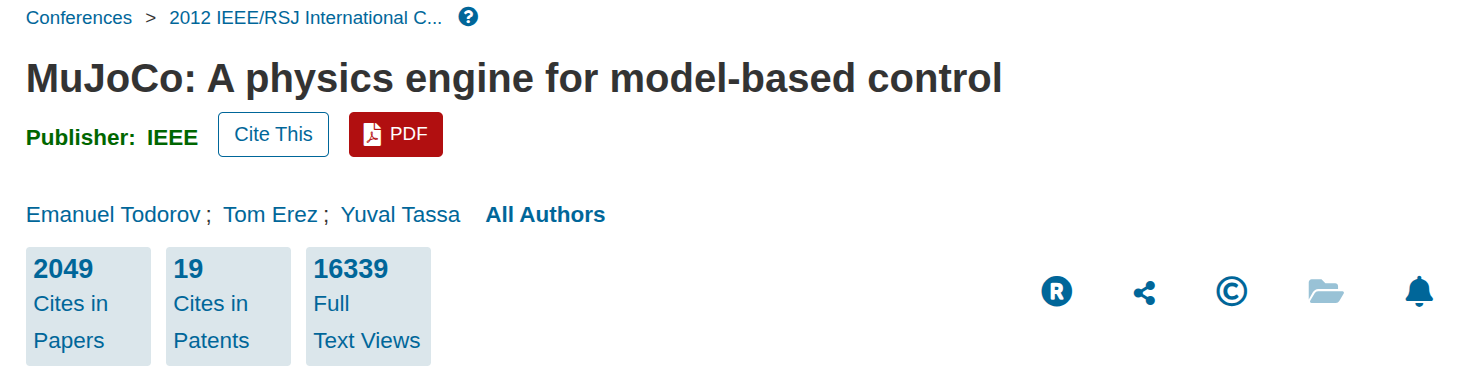
\includegraphics[width=0.5\linewidth, fbox]{images/paper-mujoco}
		\end{center}
		
		\begin{center}
			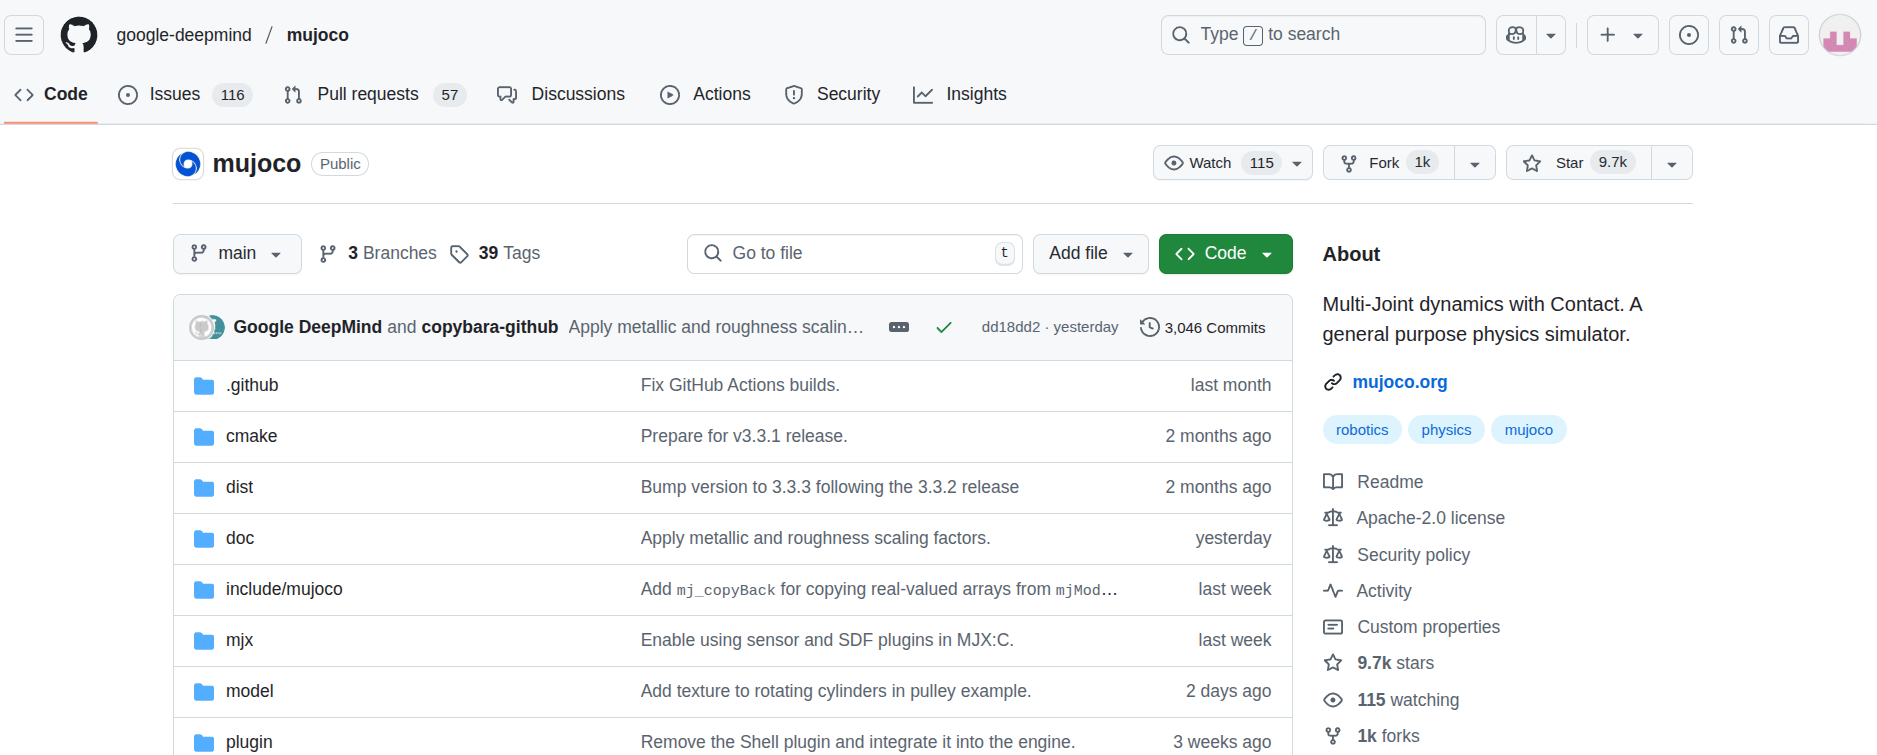
\includegraphics[width=0.7\linewidth, , fbox]{images/github-mujoco}
		\end{center}
	
	\end{frame}
	
	\begin{frame}
		\frametitle{Comparison}
			Comparisons of Simscape, MuJoCo and IsaacSim from 2015
			
			\scalebox{0.63}{

\tikzset{every picture/.style={line width=0.75pt}} %set default line width to 0.75pt        

\begin{tikzpicture}[x=0.75pt,y=0.75pt,yscale=-1,xscale=1]
	%uncomment if require: \path (0,413); %set diagram left start at 0, and has height of 413
	
	%Image [id:dp8211934472235604] 
	\draw (165.6,196.48) node  {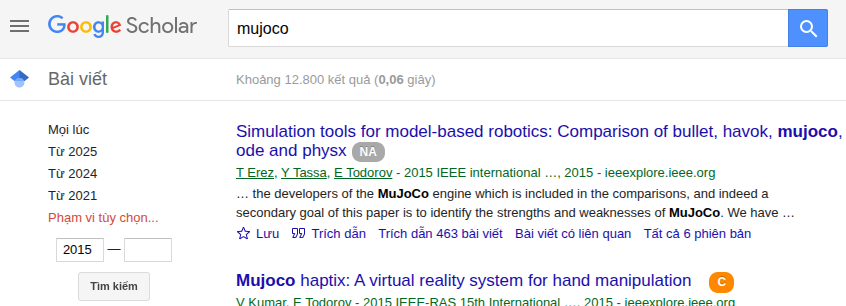
\includegraphics[width=246.9pt,height=89.3pt]{gg-mujoco-2015.png}};
	%Image [id:dp9842657245998253] 
	\draw (165.6,325.43) node  {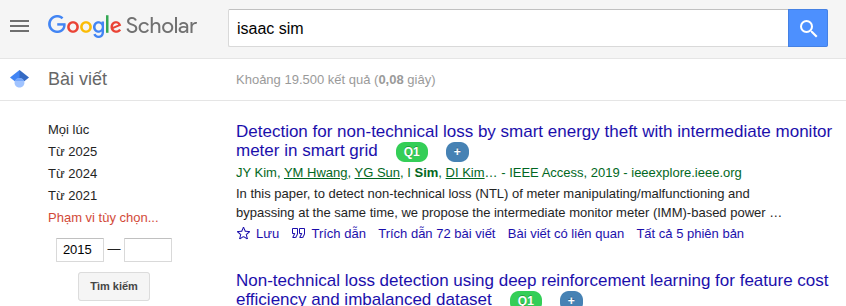
\includegraphics[width=246.9pt,height=89.3pt]{gg-isaac-2015.png}};
	%Image [id:dp2524618631997998] 
	\draw (165.6,68.88) node  {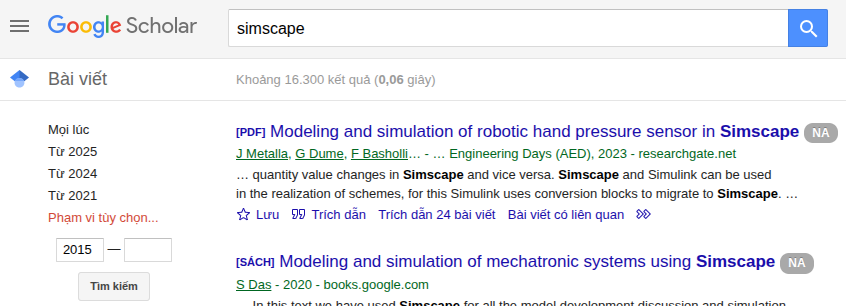
\includegraphics[width=246.9pt,height=89.3pt]{gg-simscape-2015.png}};
	%Image [id:dp5533775851298544] 
	\draw (495.6,325.43) node  {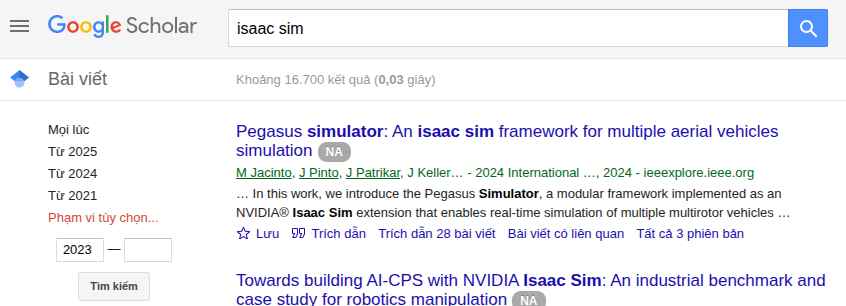
\includegraphics[width=246.9pt,height=89.3pt]{gg-isaac.png}};
	%Image [id:dp5554183262379718] 
	\draw (495.6,196.48) node  {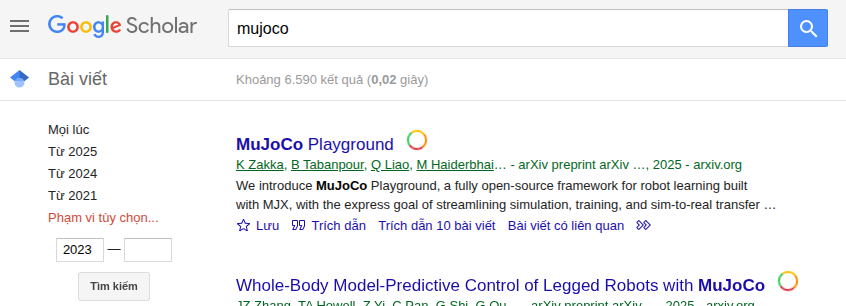
\includegraphics[width=246.9pt,height=89.3pt]{gg-mujoco.png}};
	%Image [id:dp5251444188157374] 
	\draw (495.6,68.88) node  {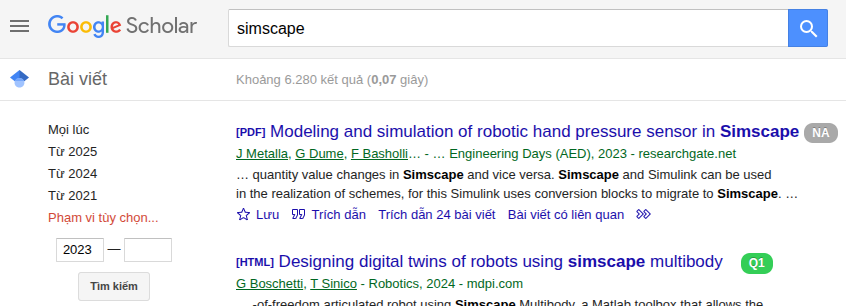
\includegraphics[width=246.9pt,height=89.3pt]{gg-simscape.png}};
	
	% Text Node
	\draw (3,387.97) node [anchor=north west][inner sep=0.75pt]   [align=left] {from 2015 - present};
	% Text Node
	\draw (332.2,387.97) node [anchor=north west][inner sep=0.75pt]   [align=left] {from 2023 - present};
	
	
\end{tikzpicture}
}
			
			IssacSim is the trend, but ...
	\end{frame}


	\begin{frame}
		\frametitle{Resources}
		\scalebox{0.8}{

\tikzset{every picture/.style={line width=0.75pt}} %set default line width to 0.75pt        

\begin{tikzpicture}[x=0.75pt,y=0.75pt,yscale=-1,xscale=1]
	%uncomment if require: \path (0,376); %set diagram left start at 0, and has height of 376
	
	%Image [id:dp7964810323222328] 
	\draw (411.78,273.28) node  {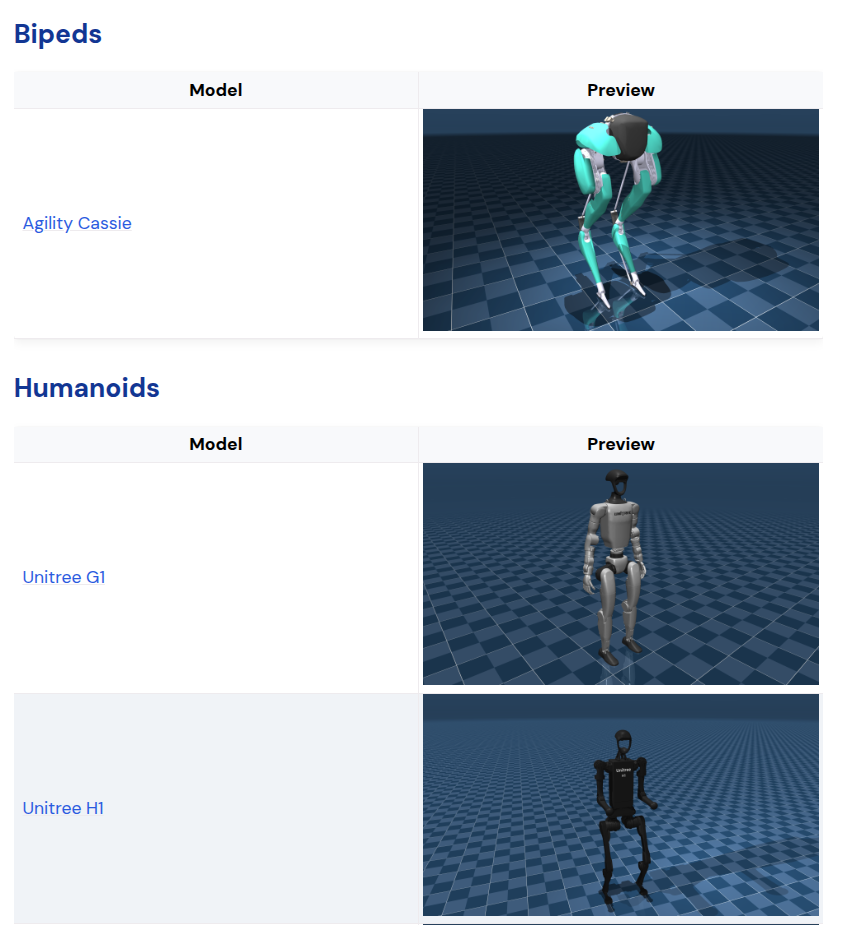
\includegraphics[width=120.83pt,height=131.81pt]{mjc-ex1.png}};
	%Image [id:dp8465926705753898] 
	\draw (89.56,97.54) node  {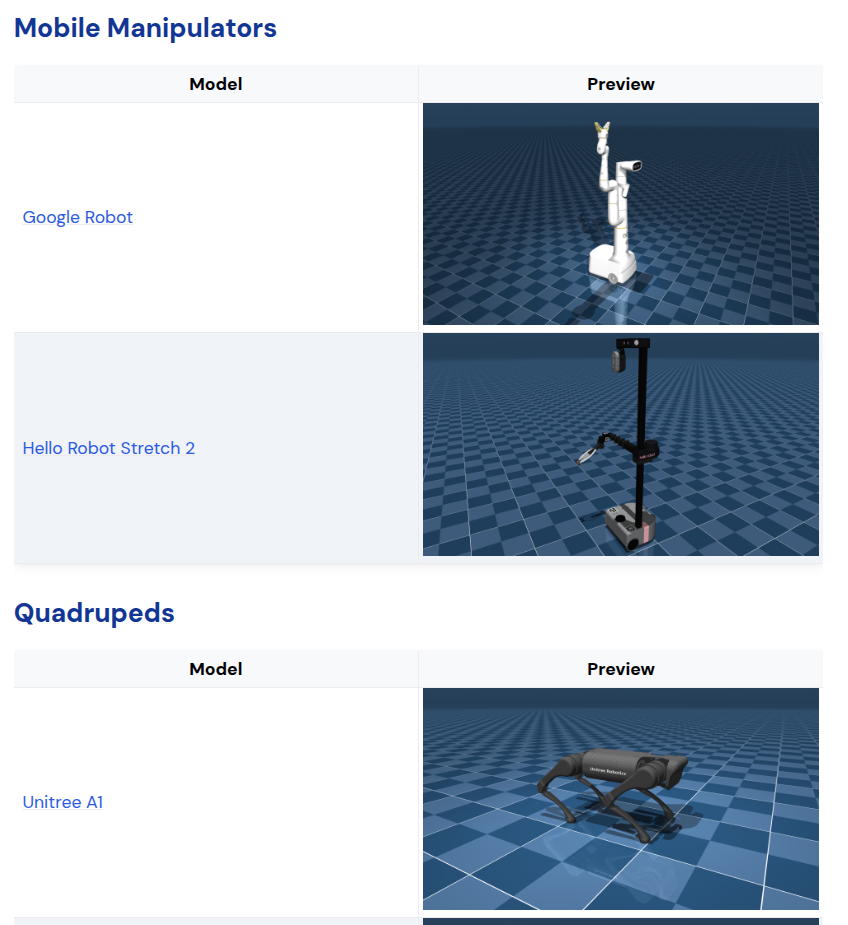
\includegraphics[width=120.83pt,height=131.81pt]{mjc-ex2.png}};
	%Image [id:dp08905471300064727] 
	\draw (89.56,273.28) node  {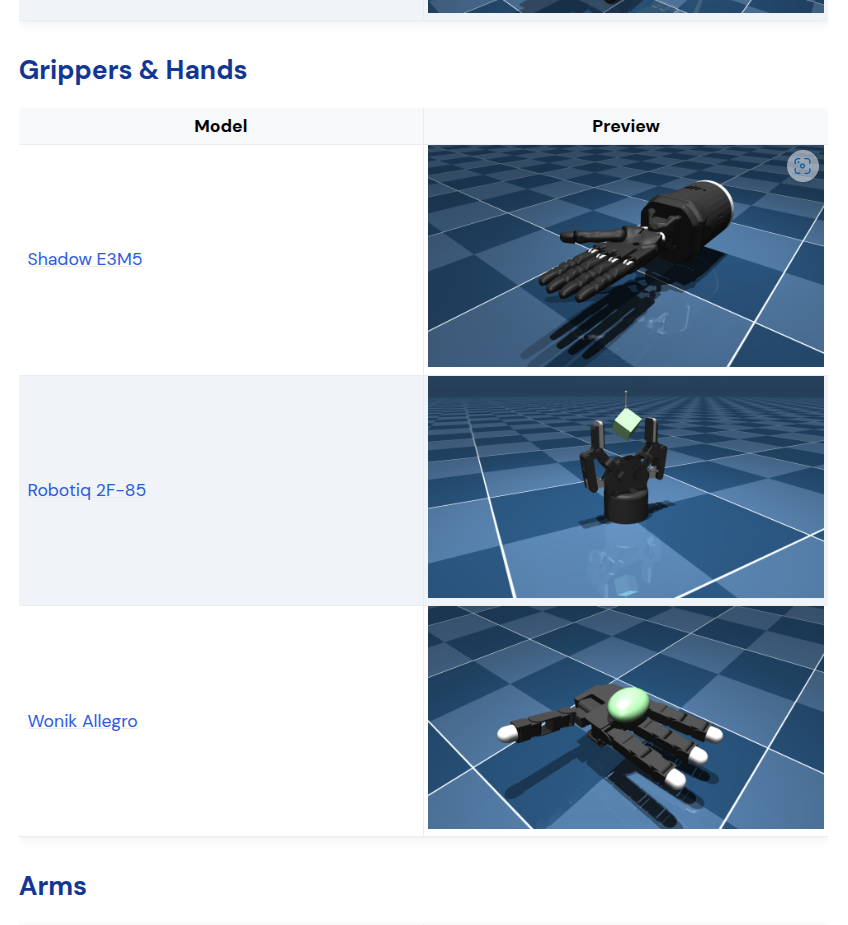
\includegraphics[width=120.83pt,height=131.81pt]{mjc-ex3.png}};
	%Image [id:dp47985912535355] 
	\draw (411.78,97.54) node  {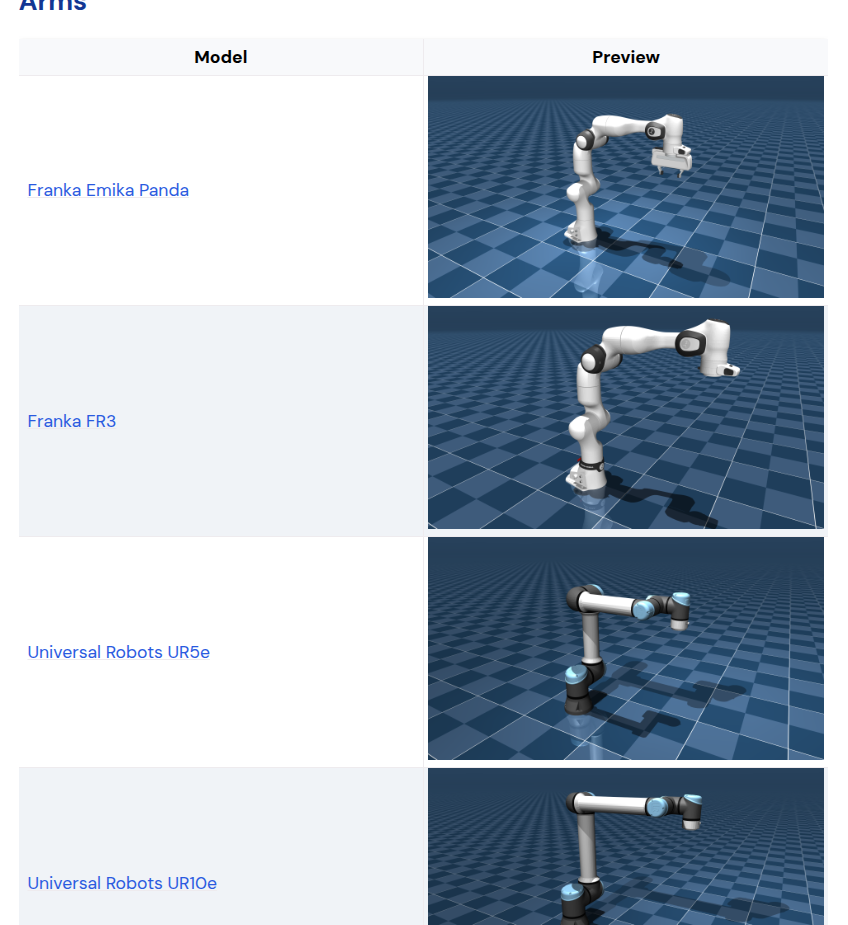
\includegraphics[width=120.83pt,height=131.81pt]{mjc-ex4.png}};
	%Image [id:dp2762099052723931] 
	\draw (250.67,273.28) node  {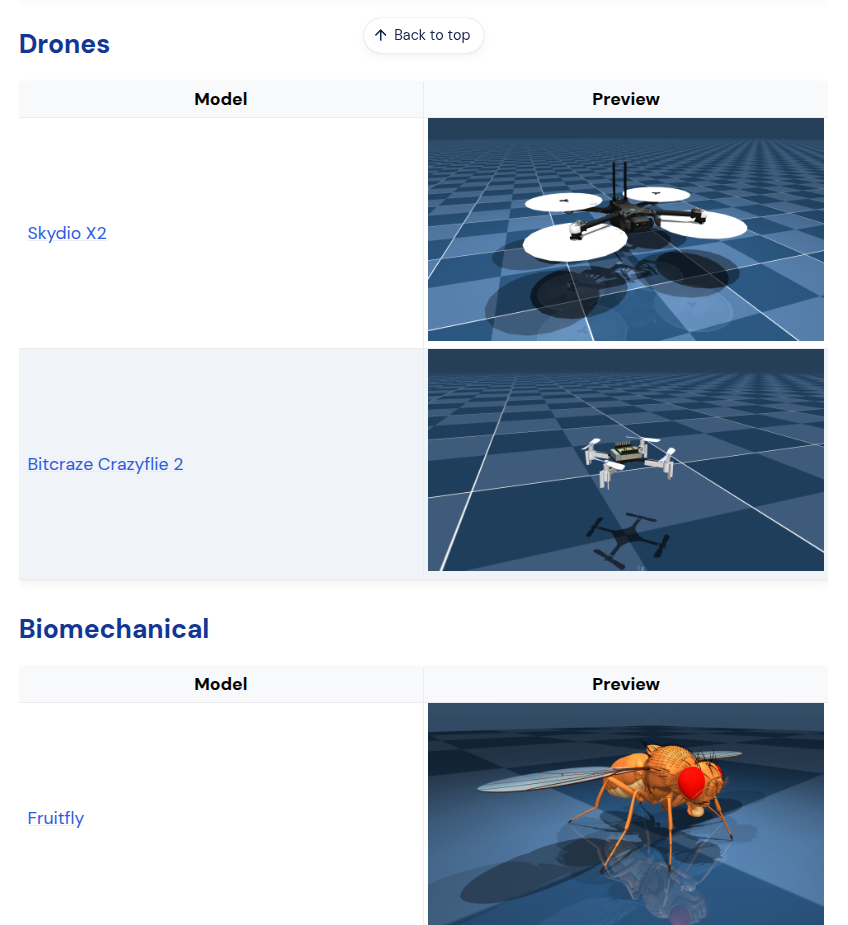
\includegraphics[width=120.83pt,height=131.81pt]{mjc-ex5.png}};
	%Image [id:dp02653722857976737] 
	\draw (250.67,97.54) node  {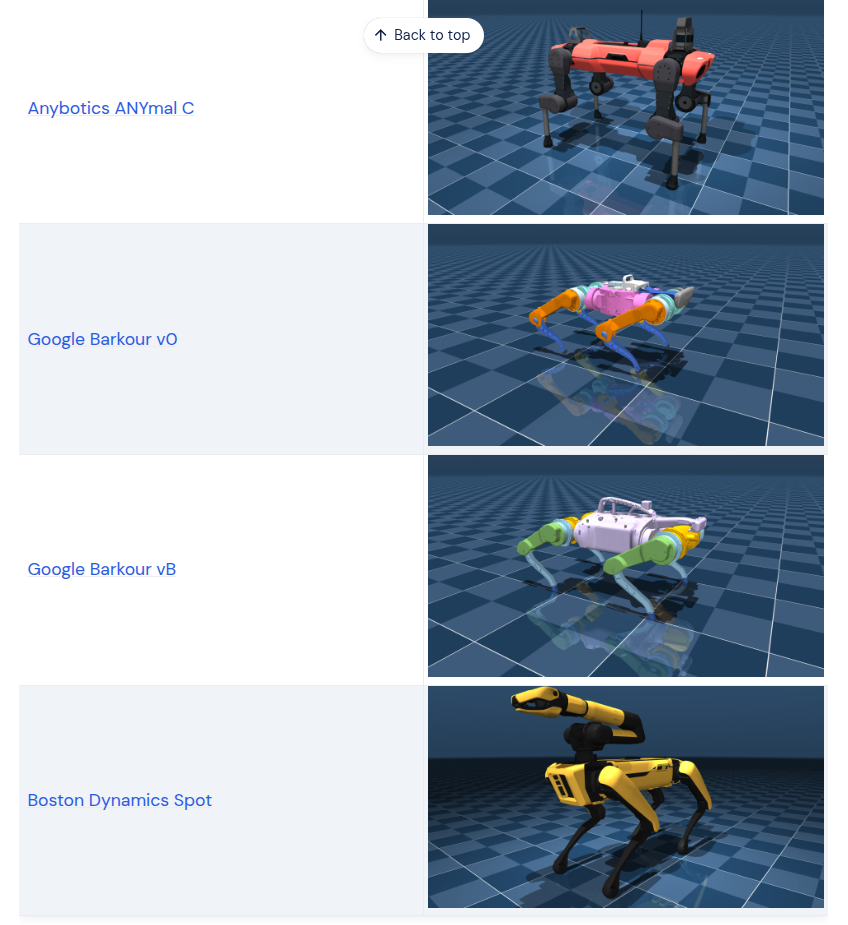
\includegraphics[width=120.83pt,height=131.81pt]{mjc-ex6.png}};
	
	
	
	
\end{tikzpicture}
}
	\end{frame}
	
	\begin{frame}[fragile]
		\frametitle{Model description}
		MuJoCo can load XML model files in its native MJCF format, as well as in the popular but more limited URDF format.
	\begin{minted}[fontsize=\footnotesize, linenos, bgcolor=gray!10]{XML}
<mujoco>
  <default class="main">
    <geom rgba="1 0 0 1"/>
    <default class="sub">
      <geom rgba="0 1 0 1"/>
    </default>
  </default>
	
  <worldbody>
    <geom type="box"/>
    <body childclass="sub">
      <geom type="ellipsoid"/>
      <geom type="sphere" rgba="0 0 1 1"/>
      <geom type="cylinder" class="main"/>
    </body>
  </worldbody>
</mujoco>
		
	\end{minted}
	\end{frame}
	
	\begin{frame}
		\frametitle{Programming}
		MuJoCo has a C API and is intended for researchers and developers. The runtime simulation module is tuned to maximize performance and operates on low-level data structures that are preallocated by the built-in XML compiler. 
		
		The Python bindings are distributed as the \texttt{mujoco} package on PyPI. These are low-level bindings that are meant to give as close to a direct access to the MuJoCo library as possible.
		
		\begin{center}
			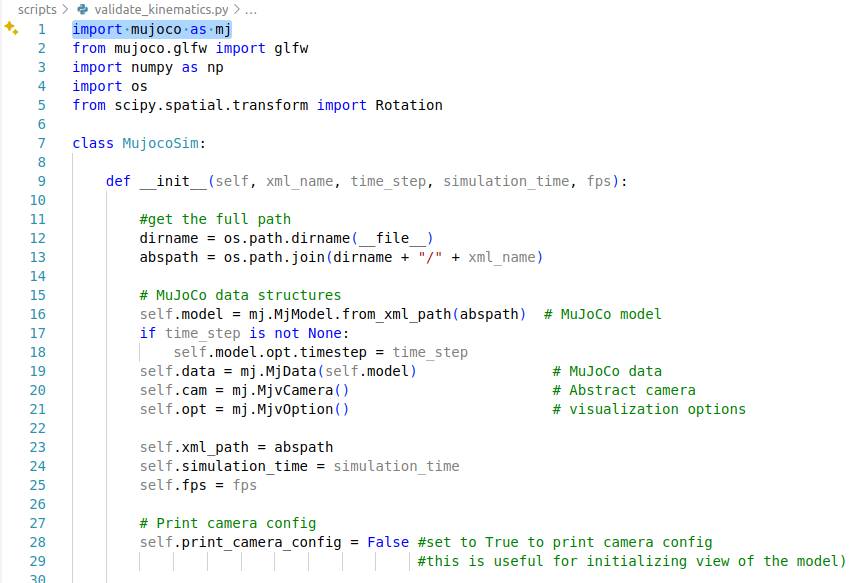
\includegraphics[width=0.7\linewidth]{images/gg-colab}
		\end{center}
	\end{frame}

	\begin{frame}
		\frametitle{Learning}
		The documents about MuJoCo could be found at
		\footnote{\href{https://mujoco.readthedocs.io/en/stable/overview.html}{https://mujoco.readthedocs.io/en/stable/overview.html}}.
		\begin{center}
			
\includegraphics[width=0.8\linewidth]{images/gg-mjc-overview}
		\end{center}
		
	\end{frame}


	
	
	% =========================================
	% =========================================
	\section{Configuration}
	% =========================================
	% =========================================
	\begin{frame}[fragile]
		\frametitle{Installation}
		\begin{minted}[fontsize=\footnotesize, linenos, bgcolor=gray!10]{XML}
pip install mujoco
		\end{minted}
	\end{frame}

	\begin{frame}
		\frametitle{Configuration}
		\begin{figure}
			\scalebox{0.6}{

\tikzset{every picture/.style={line width=0.75pt}} %set default line width to 0.75pt        

\begin{tikzpicture}[x=0.75pt,y=0.75pt,yscale=-1,xscale=1]
	%uncomment if require: \path (0,294); %set diagram left start at 0, and has height of 294
	
	%Image [id:dp6050577265750149] 
	\draw (256.6,91.52) node  {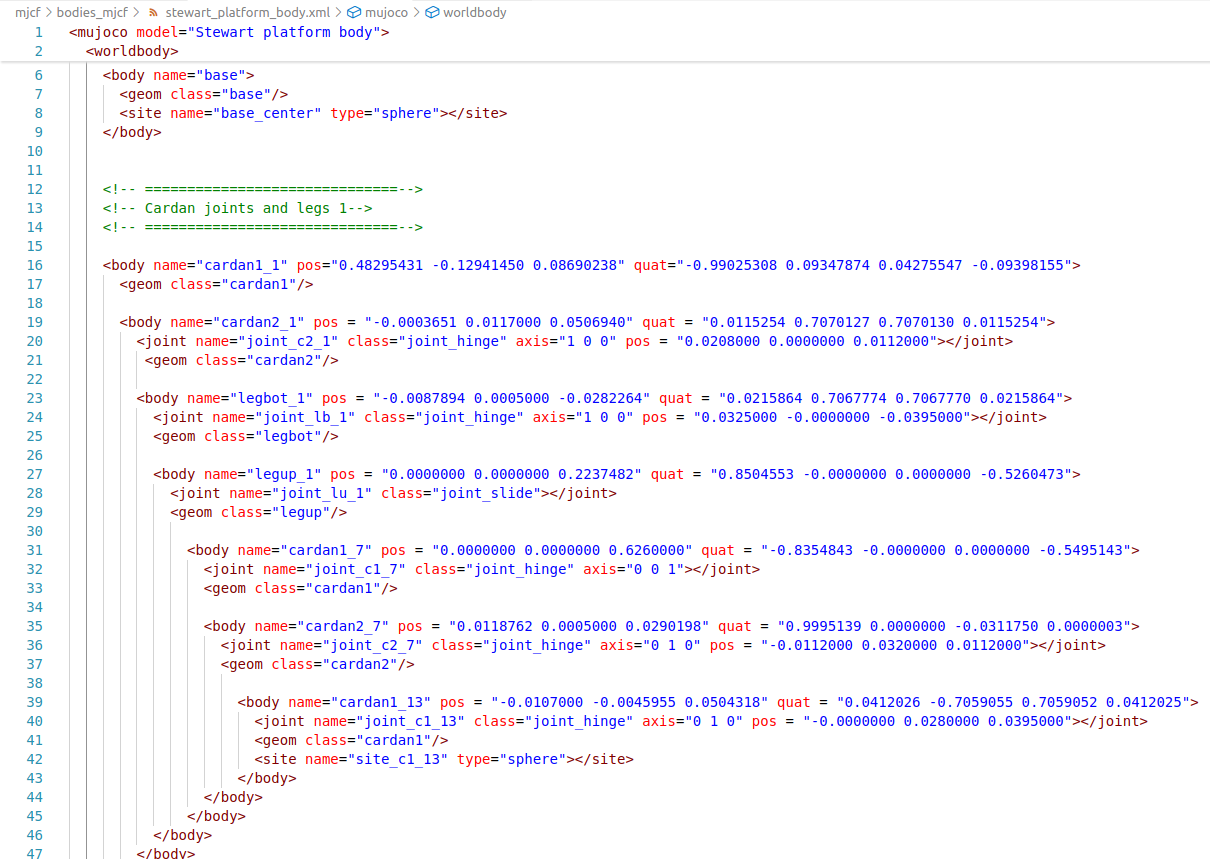
\includegraphics[width=113.4pt,height=74.88pt]{vscode-xml.png}};
	%Image [id:dp4103408524493818] 
	\draw (301.67,56.56) node  {
\includegraphics[width=18.91pt,height=17.59pt]{gg-xml.png}};
	%Shape: Rectangle [id:dp16081927472626079] 
	\draw   (181,41.6) -- (332.2,41.6) -- (332.2,141.44) -- (181,141.44) -- cycle ;
	
	%Image [id:dp9369943974675126] 
	\draw (82.6,144.7) node  {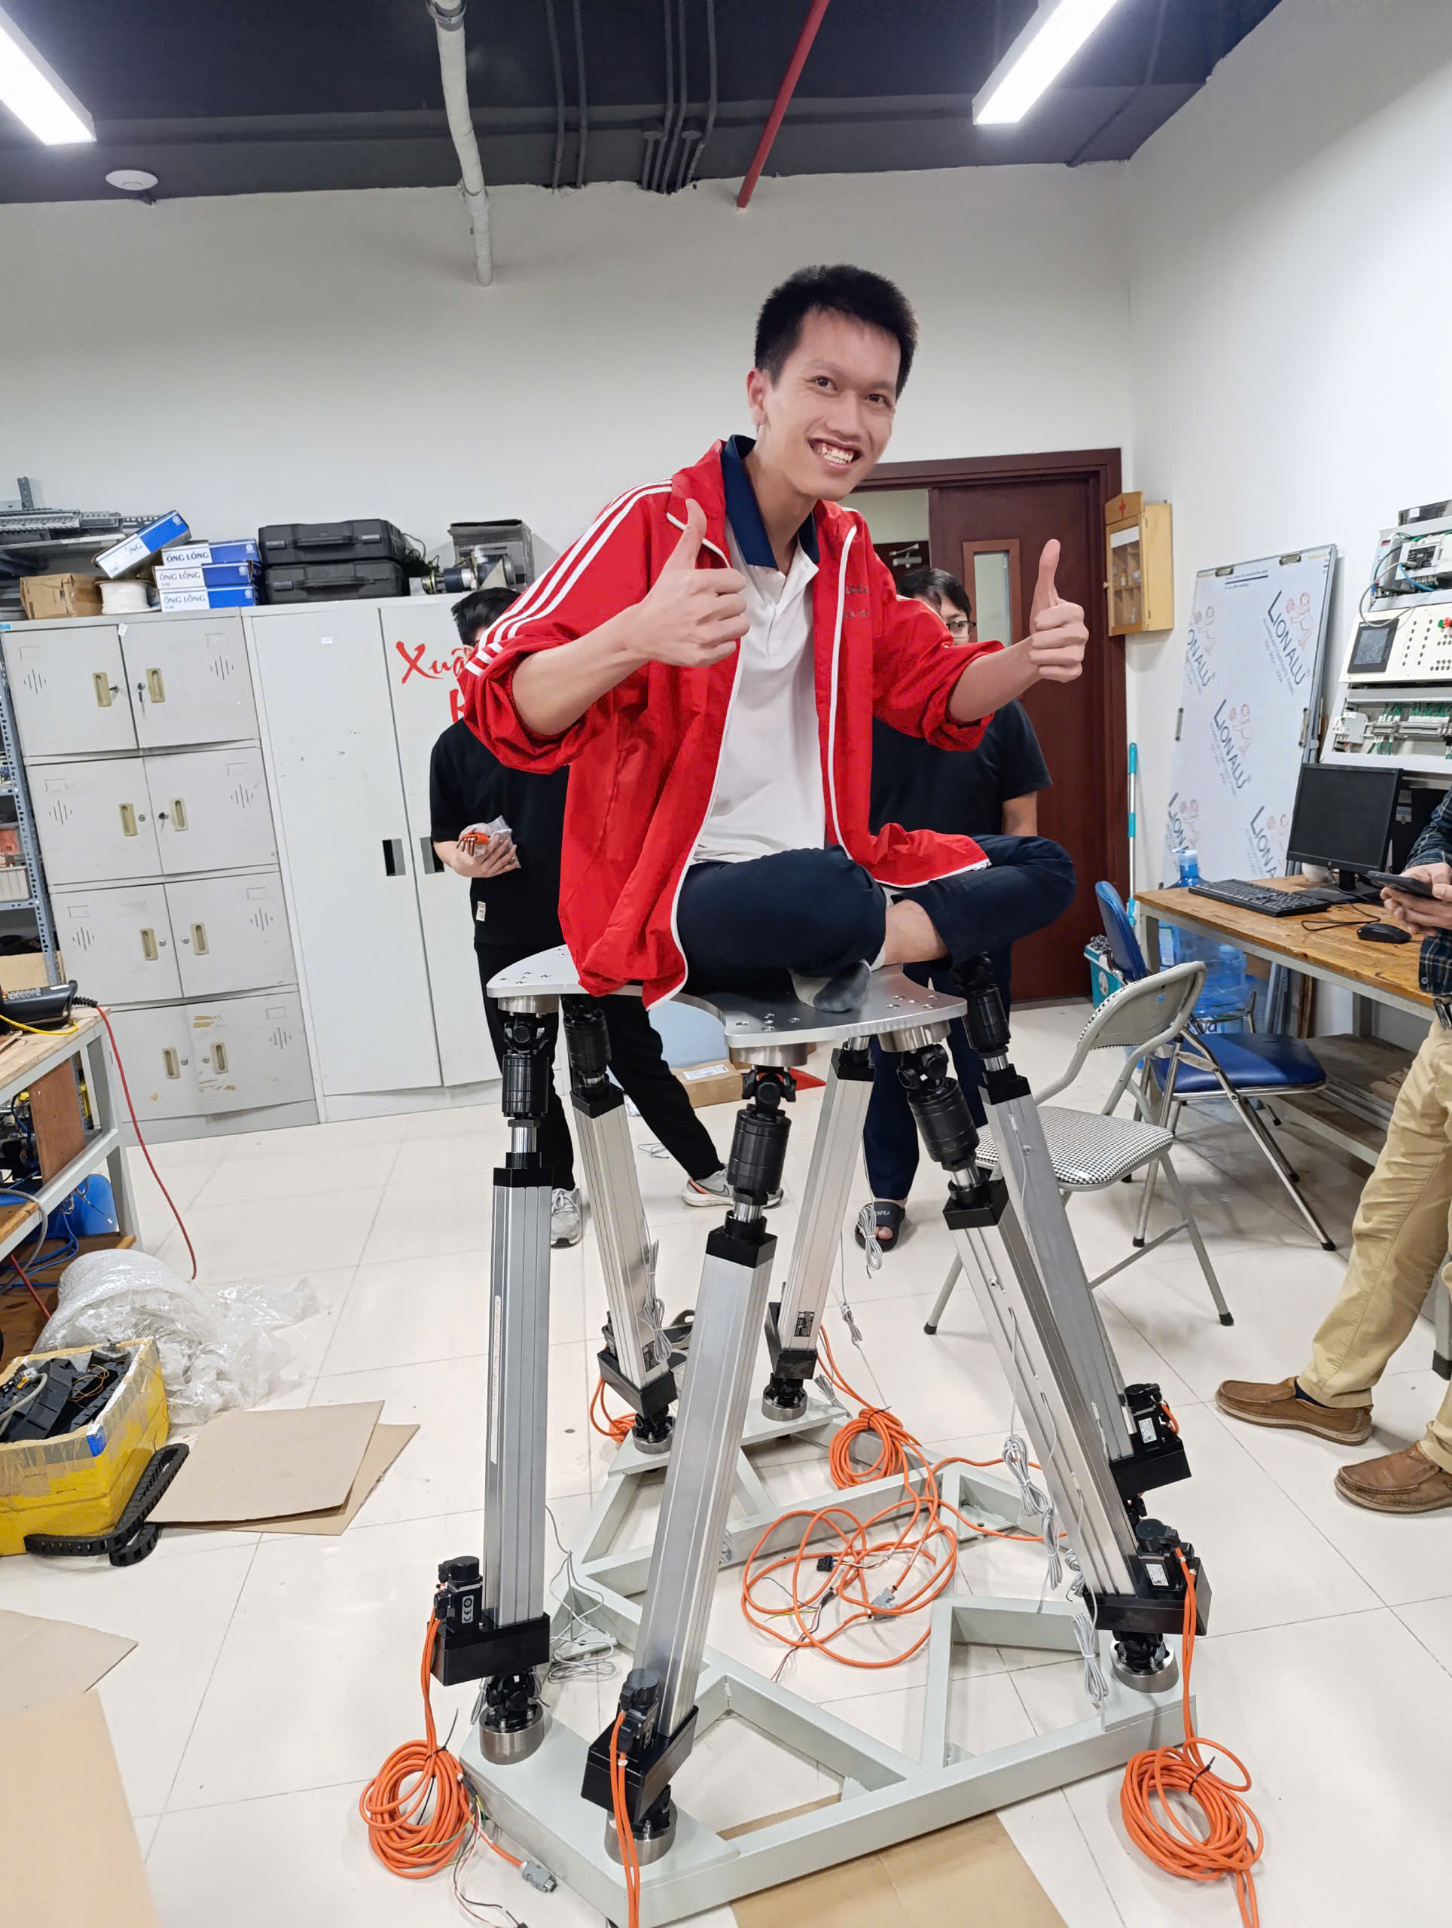
\includegraphics[width=95.4pt,height=126.15pt]{real-stewart.png}};
	%Shape: Rectangle [id:dp929363304432309] 
	\draw   (19,60.6) -- (146.2,60.6) -- (146.2,228.8) -- (19,228.8) -- cycle ;
	
	%Image [id:dp5416117995243275] 
	\draw (521.1,109.06) node  {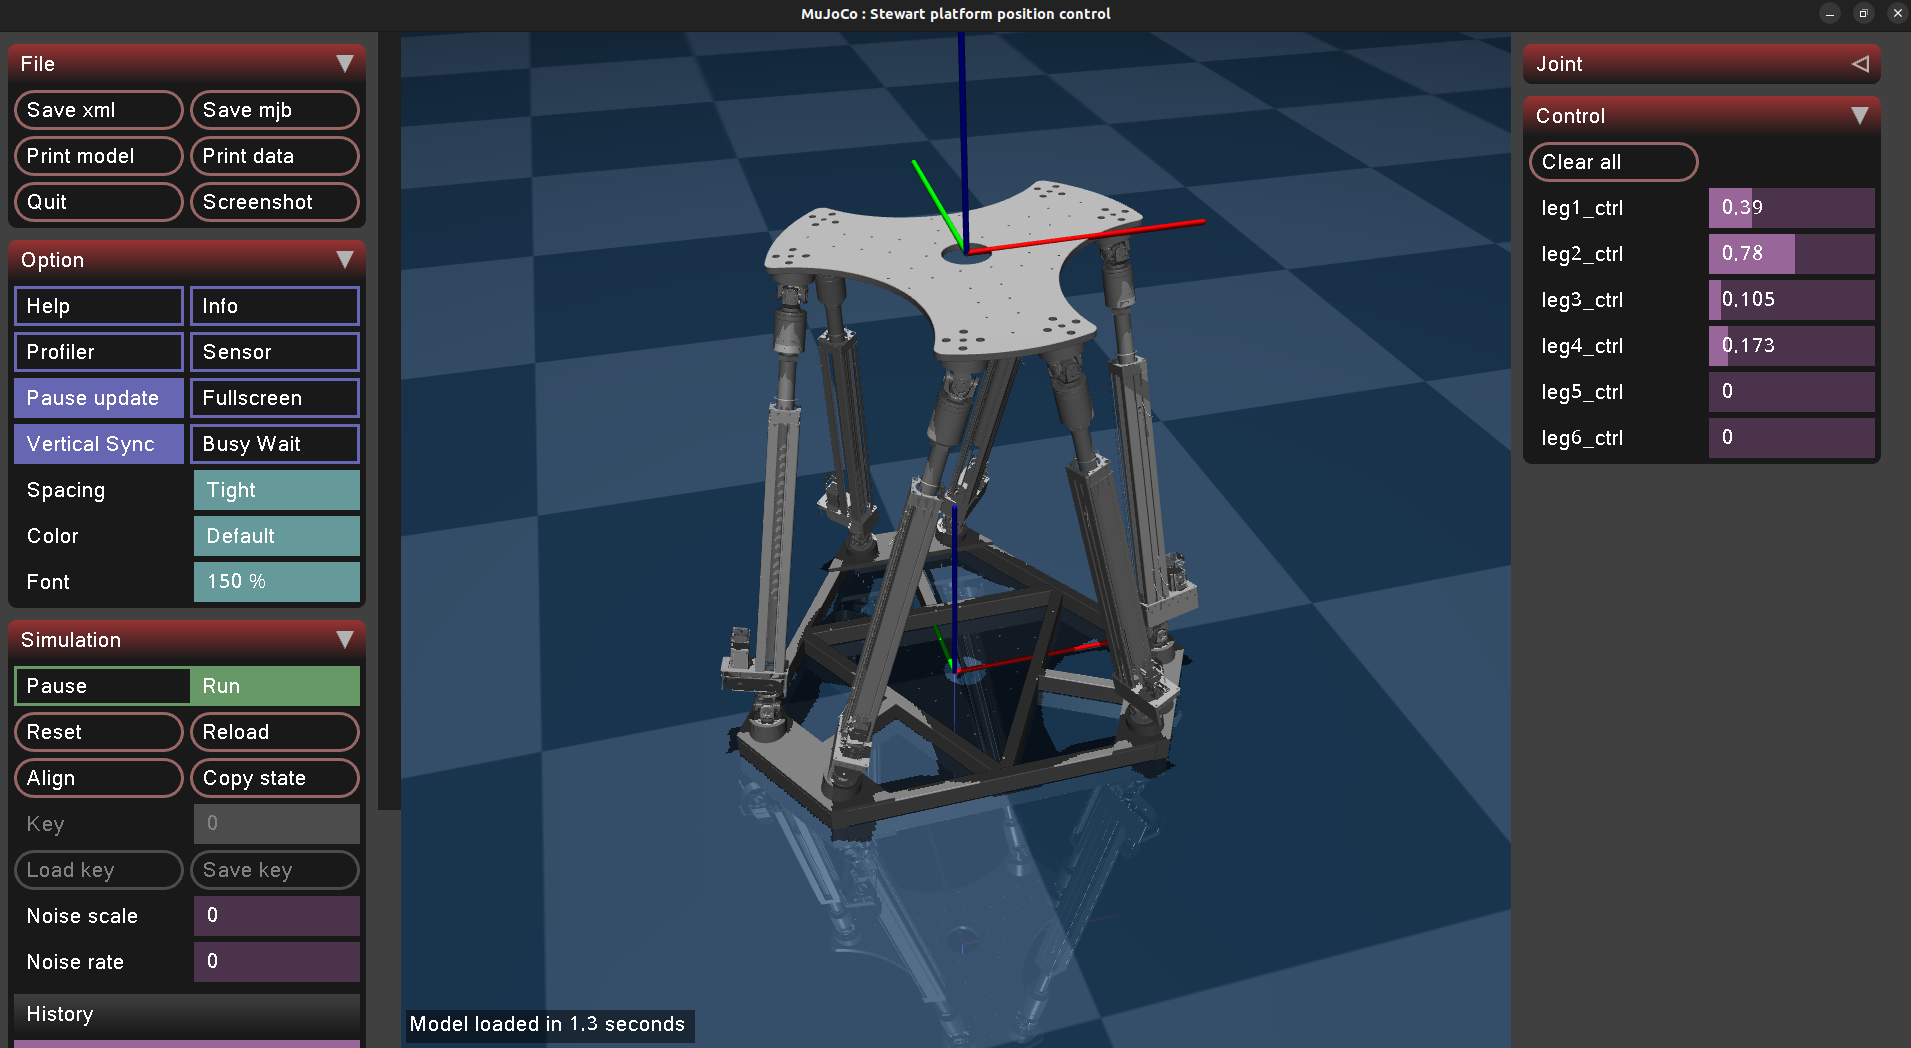
\includegraphics[width=186.15pt,height=102.09pt]{mujoco-stewart.png}};
	%Shape: Rectangle [id:dp0001749169919830207] 
	\draw   (397,41) -- (645.2,41) -- (645.2,177.11) -- (397,177.11) -- cycle ;
	
	%Rounded Rect [id:dp5884670081331446] 
	\draw   (8.2,32.6) .. controls (8.2,19.9) and (18.5,9.6) .. (31.2,9.6) -- (337.2,9.6) .. controls (349.9,9.6) and (360.2,19.9) .. (360.2,32.6) -- (360.2,256.6) .. controls (360.2,269.3) and (349.9,279.6) .. (337.2,279.6) -- (31.2,279.6) .. controls (18.5,279.6) and (8.2,269.3) .. (8.2,256.6) -- cycle ;
	%Bend Up Arrow [id:dp4779894085615144] 
	\draw   (380,254.96) -- (519.1,254.96) -- (519.1,219.02) -- (511.04,219.02) -- (525.12,199.6) -- (539.2,219.02) -- (531.14,219.02) -- (531.14,267) -- (380,267) -- cycle ;
	%Image [id:dp23296886516718363] 
	\draw (256.1,203.11) node  {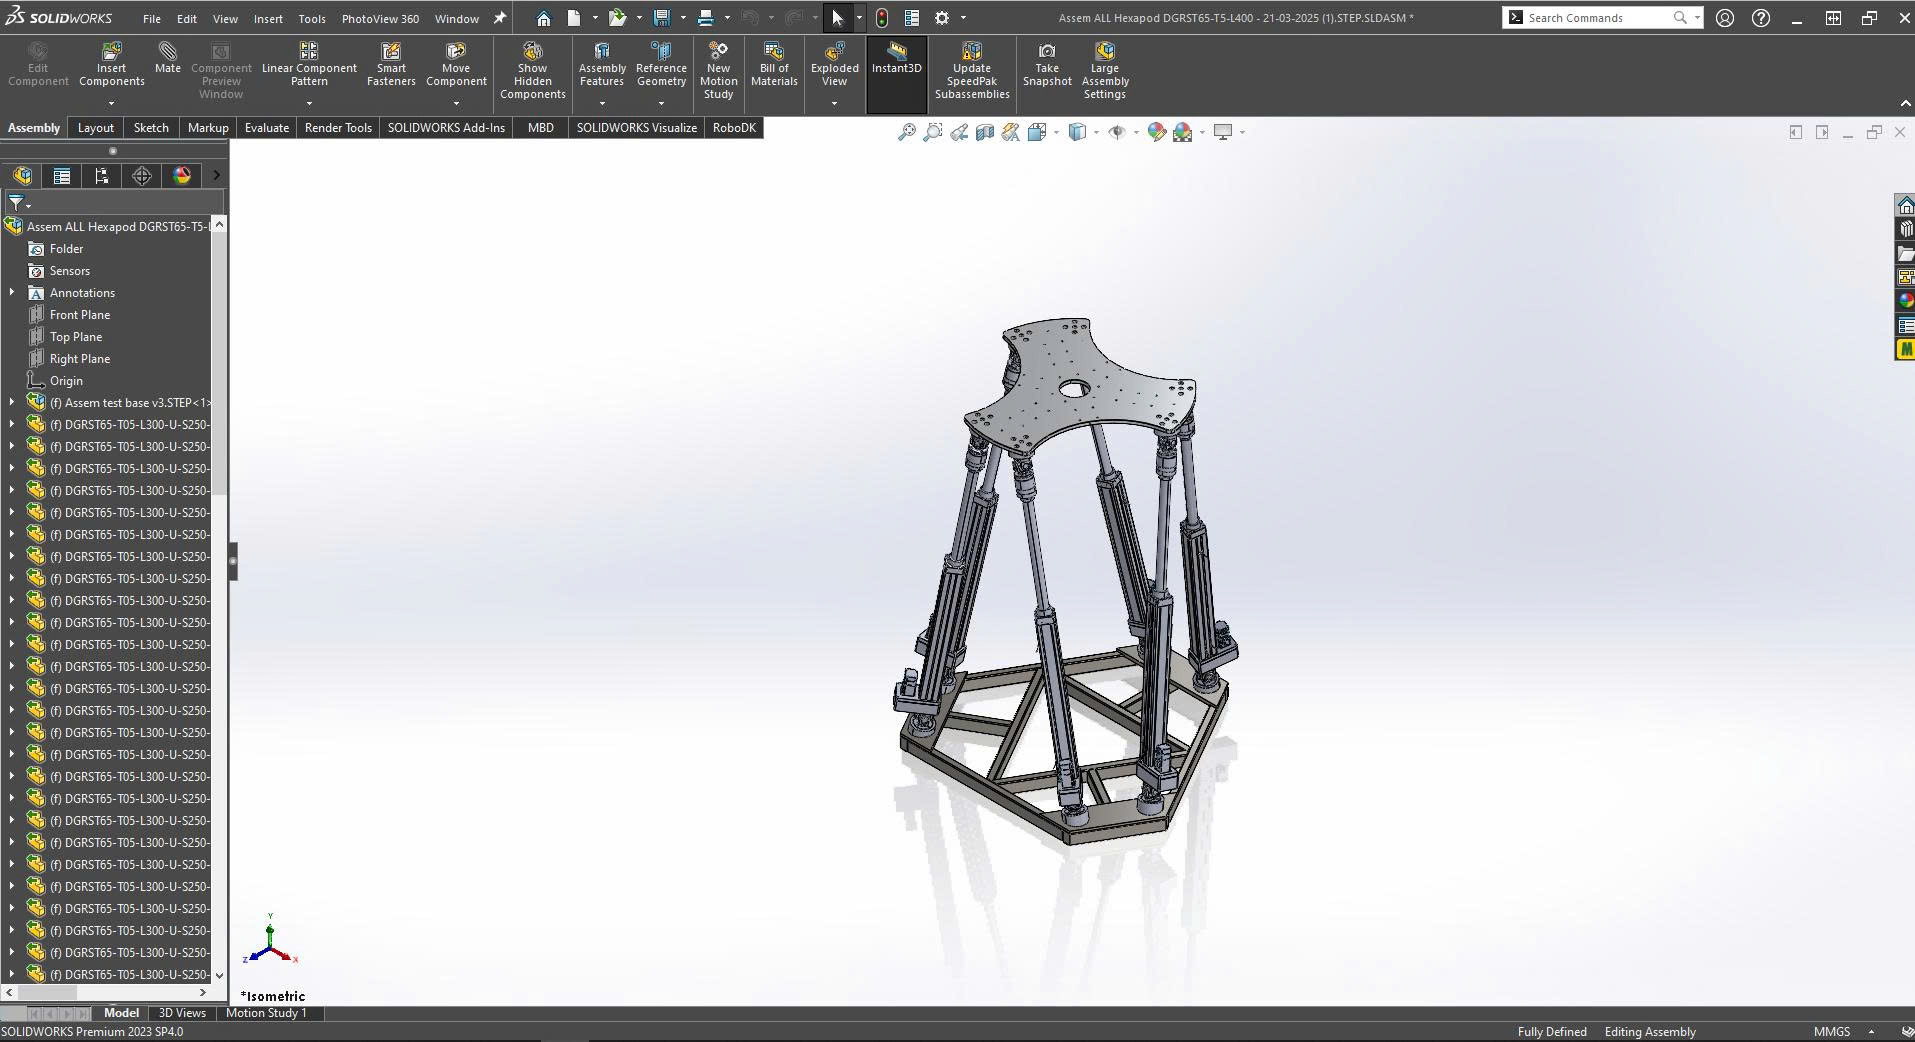
\includegraphics[width=138.15pt,height=75.17pt]{sw-stewart.jpg}};
	%Shape: Rectangle [id:dp47379488924670254] 
	\draw   (164,153) -- (348.2,153) -- (348.2,253.23) -- (164,253.23) -- cycle ;
	
	
	% Text Node
	\draw (183,38.6) node [anchor=south west] [inner sep=0.75pt]   [align=left] {xml descriptions};
	% Text Node
	\draw (166,256.23) node [anchor=north west][inner sep=0.75pt]   [align=left] {computer aided design};
	% Text Node
	\draw (21,231.8) node [anchor=north west][inner sep=0.75pt]   [align=left] {real-world model};
	% Text Node
	\draw (399,38) node [anchor=south west] [inner sep=0.75pt]   [align=left] {MuJoCo model};
	
	
\end{tikzpicture}
}
		\end{figure}
		
		Process of replicating a real-world Stewart platform model into a MuJoCo simulation environment: Starting from the real-world model, the system is first designed in a computer-aided design (CAD) software (SolidWorks, Inventor). The CAD design is then translated into XML descriptions compatible with MuJoCo. Finally, the structured XML is used to construct the MuJoCo model with the actuators, sensors, ..., enabling high-fidelity physics-based simulation and control testing.	
	\end{frame}
	

	
	% =========================================
	% =========================================
	\section{Examples}
	% =========================================
	% =========================================
		\subsection{7-DOF serial manipulator}
		
		\begin{frame}
			\frametitle{7-DOF serial manipulator}
			7-DOF serial manipulator simulation in MuJoCo, the open-source is available at \footnote{\href{https://github.com/dc-vu/mujoco_7DOFs_robot_arm_simulation.git}{https://github.com/dc-vu/mujoco\_7DOFs\_robot\_arm\_simulation.git}} (Contributor: Duc-Cuong Vu)
			\begin{center}
				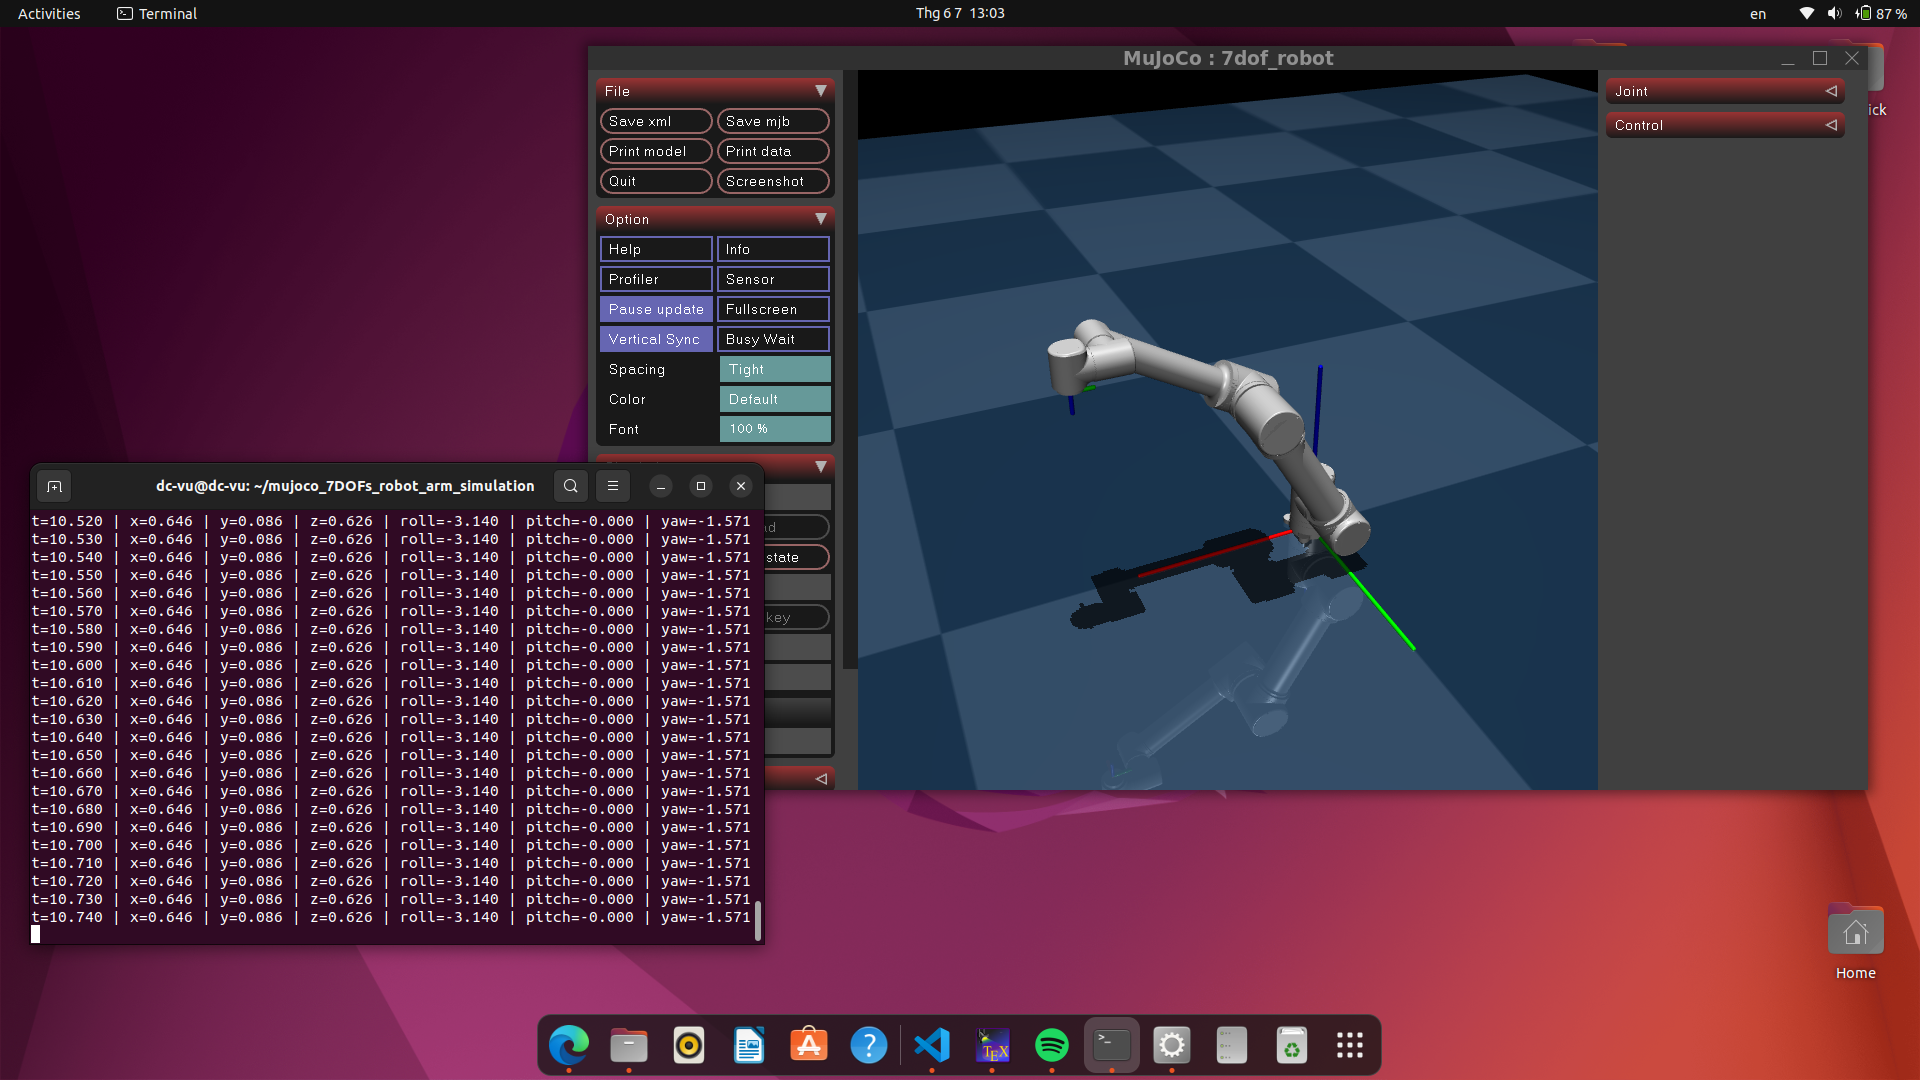
\includegraphics[width=0.9\linewidth]{images/mjc-7dof}
			\end{center}
			
		\end{frame}
	
	
		\begin{frame}[fragile]
			\frametitle{Robot definition}
			Robot XML definition
		\begin{minted}[fontsize=\footnotesize, linenos, bgcolor=gray!10]{XML}
<asset>
  <mesh name="base_mesh" file="base.stl" scale="0.001 0.001 0.001"/>
  <mesh name="motor110_mesh" file="motor110.stl" scale="0.001 0.001 0.001"/>
  <mesh name="motor70_mesh" file="motor70.stl" scale="0.001 0.001 0.001"/>
  <mesh name="link2_mesh" file="link2.stl" scale="0.001 0.001 0.001"/>
  <mesh name="link3_mesh" file="link3.stl" scale="0.001 0.001 0.001"/>
</asset>

 
<!-- Link 1 -->
  <body name="link1">
    <joint name="joint1" type="hinge" axis="0 0 1"/>
    <geom type="mesh" mesh="motor110_mesh"/>

    <!-- Link 2 -->
    <body name="link2"> 
      <joint name="joint2" type="hinge" axis="0 0 1" />
      <geom type="mesh" mesh="motor110_mesh"/>
      
      <!-- Robot tree-based definition => easy -->
      
<!-- Sensing -->
<sensor>
  <framepos name="ee_pos" objtype="body" objname="ee"/>
  <framequat name="ee_quat" objtype="body" objname="ee"/>
</sensor>
		\end{minted}
		\end{frame}
	
		\begin{frame}[fragile]
			            
			\frametitle{Inverse kinematics validation}
					\begin{minted}[fontsize=\footnotesize, linenos, bgcolor=gray!10]{python}
ee_pos = data.body("ee").xpos
eex, eey, eez = ee_pos
ee_xmat_flat = data.body("ee").xmat
ee_R = np.array(ee_xmat_flat).reshape(3, 3)
ori = R.from_matrix(ee_R).as_euler('xyz')
print(f"t={t:.3f} | x={eex:.3f} | y={eey:.3f} | z={eez:.3f} | "
	f"roll={ori[0]:.3f} | pitch={ori[1]:.3f} | yaw={ori[2]:.3f}")
# Inverse kinematics calculation here => do not straightforward
for i in range(7):
	data.joint(f"joint{i+1}").qpos = joint_demand[i] - angles_offset[i]
			\end{minted}
		
			\begin{figure}
				\scalebox{0.7}{

\tikzset{every picture/.style={line width=0.75pt}} %set default line width to 0.75pt        

\begin{tikzpicture}[x=0.75pt,y=0.75pt,yscale=-1,xscale=1]
	\fontsize{11pt}{12pt}\selectfont
	%uncomment if require: \path (0,217); %set diagram left start at 0, and has height of 217
	
	%Image [id:dp6889538666297523] 
	\draw (259,106.73) node  {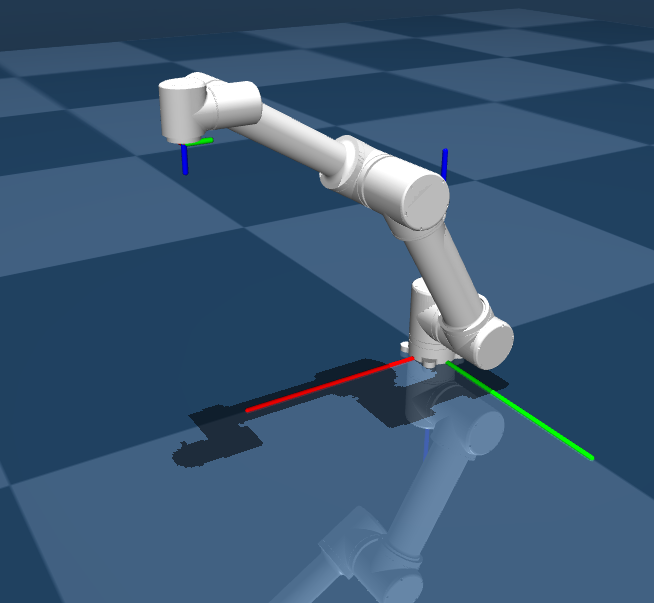
\includegraphics[width=159pt,height=146.6pt]{robot7dof.png}};
	%Curve Lines [id:da580161720299337] 
	\draw [color={rgb, 255:red, 0; green, 255; blue, 0 }  ,draw opacity=1 ]   (215,66.54) .. controls (235,121.54) and (235,180.54) .. (391,173.54) ;
	\draw [shift={(391,173.54)}, rotate = 177.43] [color={rgb, 255:red, 0; green, 255; blue, 0 }  ,draw opacity=1 ][line width=0.75]    (10.93,-3.29) .. controls (6.95,-1.4) and (3.31,-0.3) .. (0,0) .. controls (3.31,0.3) and (6.95,1.4) .. (10.93,3.29)   ;
	%Curve Lines [id:da09242711224450773] 
	\draw [color={rgb, 255:red, 0; green, 255; blue, 0 }  ,draw opacity=1 ]   (593,177.54) .. controls (640.52,157.74) and (634.13,88.94) .. (593.25,65.25) ;
	\draw [shift={(592,64.54)}, rotate = 28.71] [color={rgb, 255:red, 0; green, 255; blue, 0 }  ,draw opacity=1 ][line width=0.75]    (10.93,-3.29) .. controls (6.95,-1.4) and (3.31,-0.3) .. (0,0) .. controls (3.31,0.3) and (6.95,1.4) .. (10.93,3.29)   ;
	%Curve Lines [id:da6843282504138404] 
	\draw [color={rgb, 255:red, 0; green, 255; blue, 0 }  ,draw opacity=1 ]   (464,54.54) .. controls (429.35,28.8) and (278.07,23.64) .. (234.29,37.13) ;
	\draw [shift={(233,37.54)}, rotate = 341.57] [color={rgb, 255:red, 0; green, 255; blue, 0 }  ,draw opacity=1 ][line width=0.75]    (10.93,-3.29) .. controls (6.95,-1.4) and (3.31,-0.3) .. (0,0) .. controls (3.31,0.3) and (6.95,1.4) .. (10.93,3.29)   ;
	%Curve Lines [id:da8394696818177255] 
	\draw [color={rgb, 255:red, 0; green, 255; blue, 0 }  ,draw opacity=1 ]   (449,57.54) .. controls (389.6,44.67) and (320.4,42.58) .. (274.39,59.04) ;
	\draw [shift={(273,59.54)}, rotate = 339.72] [color={rgb, 255:red, 0; green, 255; blue, 0 }  ,draw opacity=1 ][line width=0.75]    (10.93,-3.29) .. controls (6.95,-1.4) and (3.31,-0.3) .. (0,0) .. controls (3.31,0.3) and (6.95,1.4) .. (10.93,3.29)   ;
	%Curve Lines [id:da09158135447808469] 
	\draw [color={rgb, 255:red, 0; green, 255; blue, 0 }  ,draw opacity=1 ]   (451,71.54) .. controls (391.6,89.36) and (353.76,97.38) .. (294.79,80.07) ;
	\draw [shift={(293,79.54)}, rotate = 16.7] [color={rgb, 255:red, 0; green, 255; blue, 0 }  ,draw opacity=1 ][line width=0.75]    (10.93,-3.29) .. controls (6.95,-1.4) and (3.31,-0.3) .. (0,0) .. controls (3.31,0.3) and (6.95,1.4) .. (10.93,3.29)   ;
	%Curve Lines [id:da5298341943704198] 
	\draw [color={rgb, 255:red, 0; green, 255; blue, 0 }  ,draw opacity=1 ]   (458,81.54) .. controls (421.18,116.37) and (379.42,131.39) .. (313.99,119.72) ;
	\draw [shift={(313,119.54)}, rotate = 10.3] [color={rgb, 255:red, 0; green, 255; blue, 0 }  ,draw opacity=1 ][line width=0.75]    (10.93,-3.29) .. controls (6.95,-1.4) and (3.31,-0.3) .. (0,0) .. controls (3.31,0.3) and (6.95,1.4) .. (10.93,3.29)   ;
	%Curve Lines [id:da9873811746998208] 
	\draw [color={rgb, 255:red, 208; green, 2; blue, 27 }  ,draw opacity=1 ] [dash pattern={on 4.5pt off 4.5pt}]  (295,121.54) .. controls (256.39,190.84) and (178.58,191.53) .. (134.33,170.2) ;
	\draw [shift={(133,169.54)}, rotate = 26.57] [color={rgb, 255:red, 208; green, 2; blue, 27 }  ,draw opacity=1 ][line width=0.75]    (10.93,-3.29) .. controls (6.95,-1.4) and (3.31,-0.3) .. (0,0) .. controls (3.31,0.3) and (6.95,1.4) .. (10.93,3.29)   ;
	%Curve Lines [id:da7589617847853484] 
	\draw [color={rgb, 255:red, 208; green, 2; blue, 27 }  ,draw opacity=1 ] [dash pattern={on 4.5pt off 4.5pt}]  (275,69.54) .. controls (236.58,138.49) and (183.62,135.65) .. (140.94,141.28) ;
	\draw [shift={(139,141.54)}, rotate = 352.06] [color={rgb, 255:red, 208; green, 2; blue, 27 }  ,draw opacity=1 ][line width=0.75]    (10.93,-3.29) .. controls (6.95,-1.4) and (3.31,-0.3) .. (0,0) .. controls (3.31,0.3) and (6.95,1.4) .. (10.93,3.29)   ;
	%Curve Lines [id:da25165735151019264] 
	\draw [color={rgb, 255:red, 208; green, 2; blue, 27 }  ,draw opacity=1 ] [dash pattern={on 4.5pt off 4.5pt}]  (232,44.54) .. controls (248.75,104.63) and (185.93,122.99) .. (142.95,129.26) ;
	\draw [shift={(141,129.54)}, rotate = 352.06] [color={rgb, 255:red, 208; green, 2; blue, 27 }  ,draw opacity=1 ][line width=0.75]    (10.93,-3.29) .. controls (6.95,-1.4) and (3.31,-0.3) .. (0,0) .. controls (3.31,0.3) and (6.95,1.4) .. (10.93,3.29)   ;
	%Curve Lines [id:da5507245481753484] 
	\draw [color={rgb, 255:red, 208; green, 2; blue, 27 }  ,draw opacity=1 ] [dash pattern={on 4.5pt off 4.5pt}]  (84,125.54) .. controls (72.18,112.74) and (76.85,118.37) .. (75.09,81.27) ;
	\draw [shift={(75,79.54)}, rotate = 87.06] [color={rgb, 255:red, 208; green, 2; blue, 27 }  ,draw opacity=1 ][line width=0.75]    (10.93,-3.29) .. controls (6.95,-1.4) and (3.31,-0.3) .. (0,0) .. controls (3.31,0.3) and (6.95,1.4) .. (10.93,3.29)   ;
	%Curve Lines [id:da6098588780506541] 
	\draw [color={rgb, 255:red, 208; green, 2; blue, 27 }  ,draw opacity=1 ] [dash pattern={on 4.5pt off 4.5pt}]  (215,66.54) .. controls (203.24,53.8) and (118.49,42.02) .. (89.69,50.97) ;
	\draw [shift={(88,51.54)}, rotate = 339.68] [color={rgb, 255:red, 208; green, 2; blue, 27 }  ,draw opacity=1 ][line width=0.75]    (10.93,-3.29) .. controls (6.95,-1.4) and (3.31,-0.3) .. (0,0) .. controls (3.31,0.3) and (6.95,1.4) .. (10.93,3.29)   ;
	
	% Text Node
	\draw (396,160) node [anchor=north west][inner sep=0.75pt]   [align=left] {framepos and framequad for \\getting end-effector pose};
	% Text Node
	\draw (465,58.54) node [anchor=north west][inner sep=0.75pt]   [align=left] {hinge joints values};
	% Text Node
	\draw (498,112.33) node [anchor=north west][inner sep=0.75pt]   [align=left] {inverse kinematics};
	% Text Node
	\draw (70,126) node [anchor=north west][inner sep=0.75pt]   [align=left] {forward \\kinematics};
	% Text Node
	\draw (60,53) node [anchor=north west][inner sep=0.75pt]   [align=left] {comparation};
	
	
\end{tikzpicture}}
			\end{figure}

		\end{frame}
	
	
		\begin{frame}[fragile]
			\frametitle{Remaining problems}
			.\begin{itemize}
				\item The inverse kinematics is not real-time, because an optimization problem is used for solving the joint states
				\begin{minted}[fontsize=\footnotesize, linenos, bgcolor=gray!10]{python}
def levenberg_marquardt_ik_dh(q_init, desired_pose):
  result = least_squares(
  ik_loss, 	# the coss  function
  q_init, 	# initial guess
  args=(desired_pose,), 
  method='trf',  # Change to 'lm' if you want to use Levenberg-Marquardt
  ftol=1e-6,     # Tolerance for the cost function
  xtol=1e-6,     # Tolerance for the solution
  gtol=1e-6,     # Tolerance for the gradient
  max_nfev=200  # Maximum number of function evaluations
  )
  return result.x, result.cost
				\end{minted}
				This function is implemented in Python, the solver is trust region method or Levenberg-Marquardt. Thus the real-time purpose is not guaranteed. This problem could be addressed by utilizing the C code in the remaining part of this talk.
				\item Need actuators
			\end{itemize}
		\end{frame}
	
	
		\subsection{6-DOF parallel mechanisms}
			\begin{frame}
				\frametitle{6-DOF parallel mechanisms - Stewart platform}
				Stewart platform simulation in MuJoCo, the open-source is not available.
				
				(Contributors: Viet Khanh Nguyen, Duc Cuong Vu)
				
				\begin{center}
					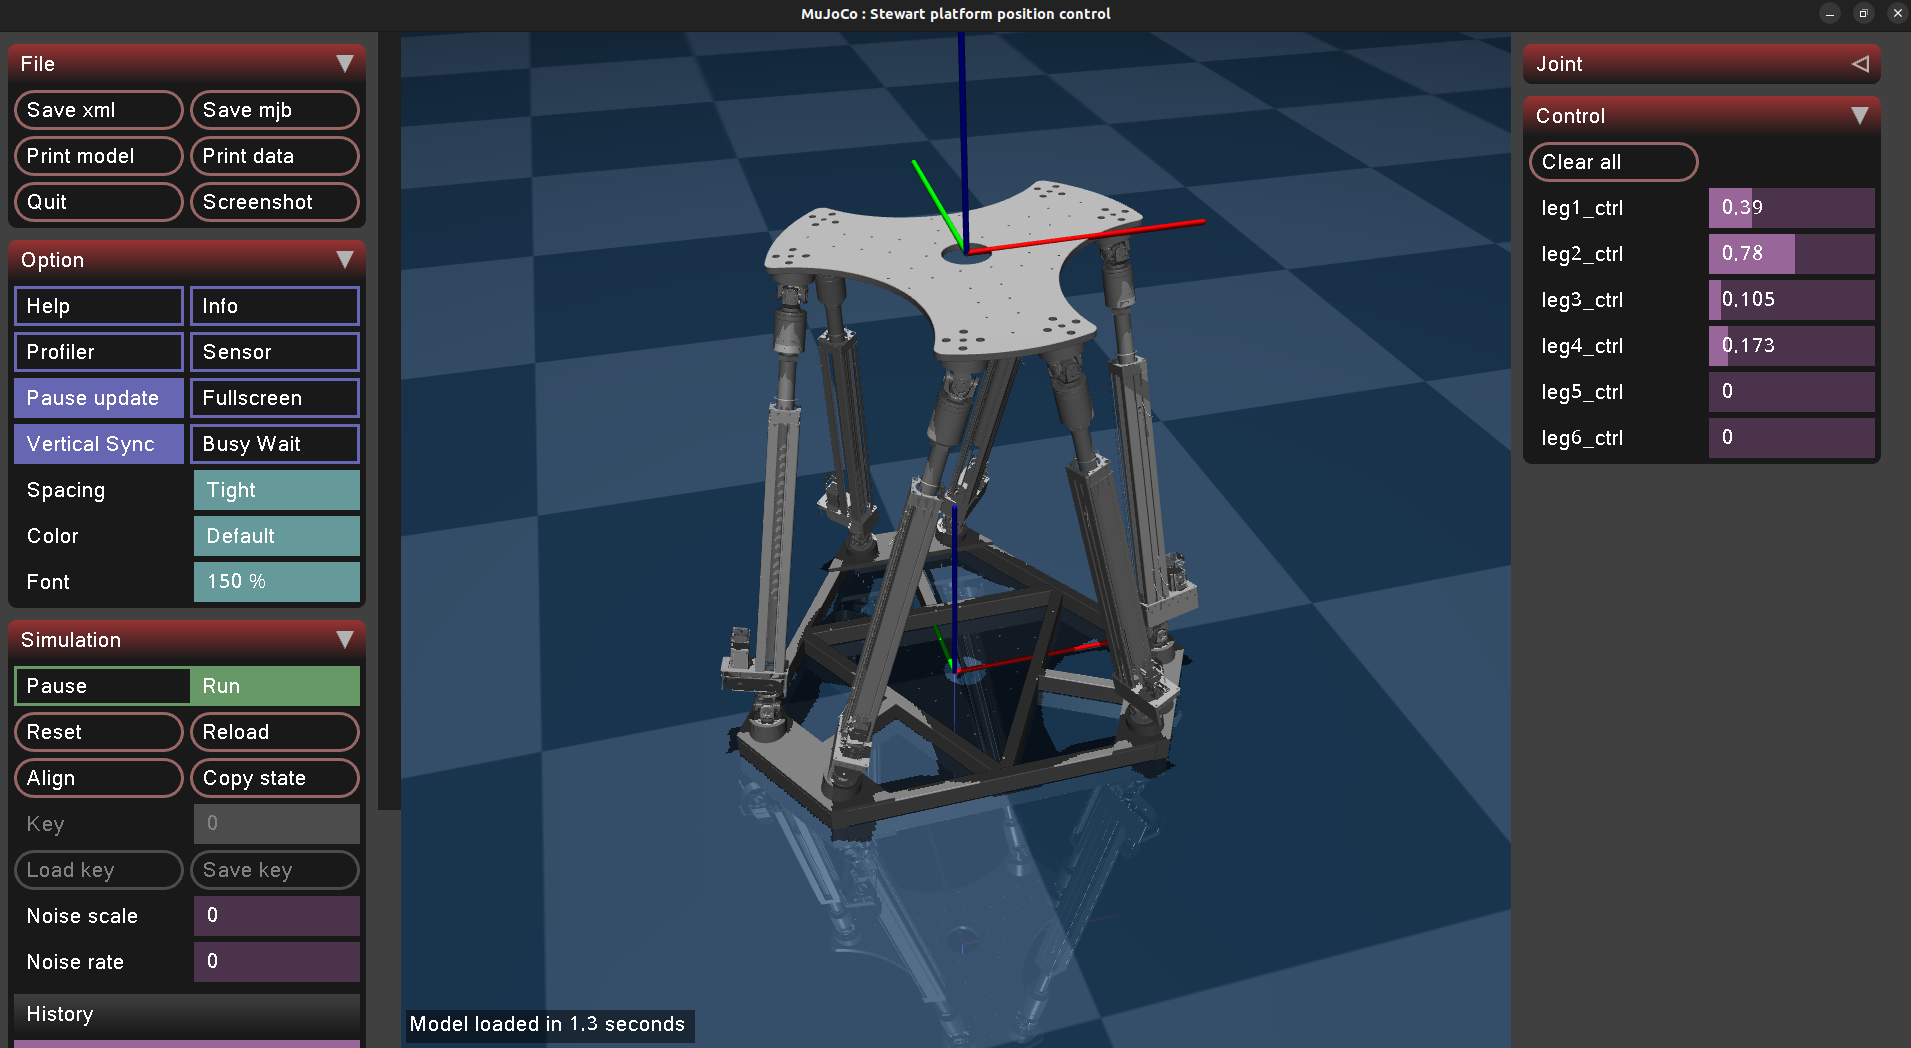
\includegraphics[width=0.9\linewidth]{mujoco-stewart}
				\end{center}
				
			\end{frame}
		
		
		
			\begin{frame}[fragile]
				\frametitle{Closed loop kinematics chain}
				\begin{figure}
					\scalebox{0.7}{

\tikzset{every picture/.style={line width=0.75pt}} %set default line width to 0.75pt        

\begin{tikzpicture}[x=0.75pt,y=0.75pt,yscale=-1,xscale=1]
	%uncomment if require: \path (0,265); %set diagram left start at 0, and has height of 265
	
	%Shape: Ellipse [id:dp7551326114257342] 
	\draw   (75.79,147.86) .. controls (81.98,142.31) and (103.89,156.65) .. (124.72,179.88) .. controls (145.54,203.12) and (157.41,226.46) .. (151.21,232.01) .. controls (145.02,237.56) and (123.11,223.23) .. (102.28,199.99) .. controls (81.46,176.75) and (69.59,153.42) .. (75.79,147.86) -- cycle ;
	%Shape: Ellipse [id:dp03803498476554046] 
	\draw   (151.21,232.01) .. controls (143.32,229.37) and (148.16,193.64) .. (162.02,152.21) .. controls (175.87,110.77) and (193.5,79.32) .. (201.39,81.95) .. controls (209.28,84.59) and (204.44,120.32) .. (190.59,161.76) .. controls (176.73,203.2) and (159.1,234.65) .. (151.21,232.01) -- cycle ;
	%Shape: Ellipse [id:dp25139516998021827] 
	\draw   (151.21,232.01) .. controls (147.46,224.59) and (167.65,206.82) .. (196.31,192.33) .. controls (224.97,177.84) and (251.25,172.11) .. (255.01,179.53) .. controls (258.76,186.96) and (238.57,204.72) .. (209.9,219.21) .. controls (181.24,233.71) and (154.96,239.43) .. (151.21,232.01) -- cycle ;
	%Shape: Ellipse [id:dp5445438337062236] 
	\draw   (201.39,81.95) .. controls (208.68,77.95) and (226.57,96.51) .. (241.36,123.41) .. controls (256.14,150.31) and (262.21,175.36) .. (254.92,179.37) .. controls (247.63,183.37) and (229.74,164.82) .. (214.96,137.92) .. controls (200.17,111.01) and (194.1,85.96) .. (201.39,81.95) -- cycle ;
	%Shape: Ellipse [id:dp17386590304939553] 
	\draw   (75.79,147.86) .. controls (67.88,145.22) and (67.77,124.19) .. (75.56,100.91) .. controls (83.35,77.62) and (96.08,60.88) .. (103.99,63.53) .. controls (111.9,66.18) and (112.01,87.2) .. (104.22,110.49) .. controls (96.43,133.78) and (83.7,150.51) .. (75.79,147.86) -- cycle ;
	%Shape: Ellipse [id:dp2638569941795088] 
	\draw   (103.54,64.32) .. controls (105.32,56.19) and (128.49,54.36) .. (155.29,60.23) .. controls (182.09,66.1) and (202.38,77.44) .. (200.6,85.57) .. controls (198.82,93.7) and (175.65,95.53) .. (148.85,89.66) .. controls (122.05,83.79) and (101.77,72.45) .. (103.54,64.32) -- cycle ;
	
	%Image [id:dp4637388297623295] 
	\draw (449.85,149.94) node  {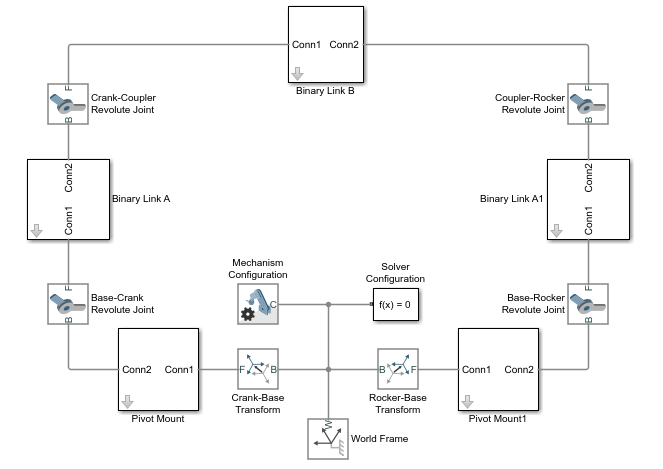
\includegraphics[width=218.28pt,height=154.41pt]{simscape-close-loop.png}};
	%Image [id:dp5015666519585665] 
	\draw (449.17,127.32) node  {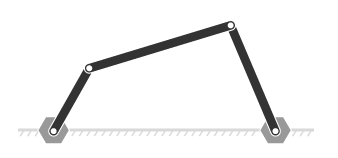
\includegraphics[width=85.25pt,height=39.85pt]{simscape-ex-closedloop.png}};
	%Shape: Ellipse [id:dp9896253160830154] 
	\draw  [color={rgb, 255:red, 255; green, 0; blue, 0 }  ,draw opacity=1 ] (389,69.94) .. controls (389,53.96) and (416.53,41) .. (450.5,41) .. controls (484.47,41) and (512,53.96) .. (512,69.94) .. controls (512,85.92) and (484.47,98.88) .. (450.5,98.88) .. controls (416.53,98.88) and (389,85.92) .. (389,69.94) -- cycle ;
	
	% Text Node
	\draw (103.56,164.12) node [anchor=north west][inner sep=0.75pt]  [rotate=-50.29] [align=left] {Link 1};
	% Text Node
	\draw (186.57,204.8) node [anchor=north west][inner sep=0.75pt]  [rotate=-333.98] [align=left] {Link 3};
	% Text Node
	\draw (73.68,120.6) node [anchor=north west][inner sep=0.75pt]  [rotate=-296.79] [align=left] {Link 3};
	% Text Node
	\draw (96,243) node [anchor=north west][inner sep=0.75pt]   [align=left] {Inertial coordinate};
	% Text Node
	\draw (115.9,58.87) node [anchor=north west][inner sep=0.75pt]  [rotate=-13.17] [align=left] {End effector};
	% Text Node
	\draw (159.34,177.84) node [anchor=north west][inner sep=0.75pt]  [rotate=-288.75] [align=left] {Link 2};
	% Text Node
	\draw (226.74,113.17) node [anchor=north west][inner sep=0.75pt]  [rotate=-61.48] [align=left] {Link 4};
	% Text Node
	\draw (64,32) node [anchor=north west][inner sep=0.75pt]   [align=left] {closed loop kinematic chain};
	% Text Node
	\draw (306,11) node [anchor=north west][inner sep=0.75pt]   [align=left] {"Which ensures that the connection is valid?};
	
	
\end{tikzpicture}}
				\end{figure}
			
				The parallel mechanisms could be described in MuJoCo by equality attribute as follows
				\begin{minted}[fontsize=\footnotesize, linenos, bgcolor=gray!10]{python}
<mujoco model="Parallel mechanisms equality">
  <equality>
    <weld name="w_1" site1="site1" site2="site2"></weld>
    <weld name="w_2" site1="site2" site2="site4"></weld>
  </equality>
</mujoco>
				\end{minted}
			\end{frame}
		
		
			
			\begin{frame}[fragile]
				\frametitle{Optimization-based kinematics - (ctypes in Python - C code for real-time implementation)}
				The algorithm is introduced in \textit{2.2. Kinematics analysis} of the publication \footnote{Vu, D. C., Nguyen, T. L., \& Nguyen, D. H. (2025). A novel approach of Consensus-based Finite-time Distributed Sliding Mode Control for Stewart platform manipulators motion tracking. Results in Engineering, 25, 103872.}
				\begin{center}
					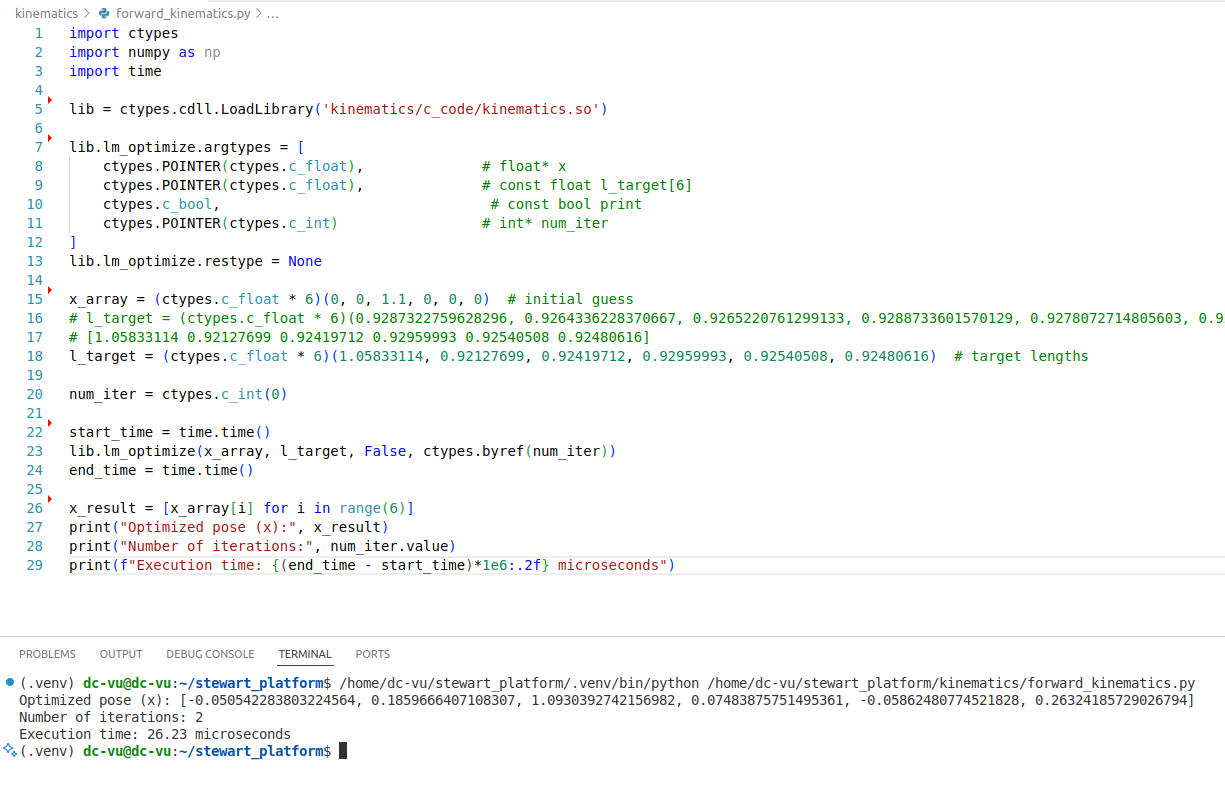
\includegraphics[width=1\linewidth]{images/vscode-fk-stewart}
				\end{center}
			\end{frame}
		
			\begin{frame}[fragile]
				\frametitle{Dynamics control}
				
				Control purpose $\to$ \textbf{The upper platform track a reference}
				
				From the desired pose of the upper platform, by the inverse kinematics, the desired length of the actuators is calculated.
				
				In the aim of this seminar, a simple PID controller is design to control the length of the actuators. 
				
					\begin{minted}[fontsize=\footnotesize, linenos, bgcolor=gray!10]{python}
# Get data from sensors ...
sensor_value = np.array([
  data.sensor('leg1_len_sensor').data,
  data.sensor("leg2_len_sensor").data,
  ...
  ]).reshape(-1) + self.legs_offset
  
# Define the controller (PID in this case) ...
self.controller = StewartPlatformPIDController(Kp, Ki, Kd, self.time_step )
 
# Apply the control signal to the model via data.ctrl
data.ctrl = self.controller.solve(errors)
					\end{minted}
			\end{frame}
		
		
			\begin{frame}[fragile]
				\frametitle{Peripherals connection}
			
			Get pose of the joystick as the references values of the upper platform.
				\begin{minted}[fontsize=\footnotesize, linenos, bgcolor=gray!10]{python}
import pygame
pygame.init()
pygame.joystick.init()

roll = normalize_euler_workingspace(round_to_step(self.joystick.get_axis(0)))
pitch = -normalize_euler_workingspace(round_to_step(self.joystick.get_axis(1)))
yaw = -normalize_euler_workingspace(round_to_step(self.joystick.get_axis(5)))
	
z = normalize_pos_workingspace(round_to_step(self.joystick.get_axis(2)))
y = normalize_pos_workingspace(round_to_step(self.joystick.get_axis(3)))
x = normalize_pos_workingspace(round_to_step(self.joystick.get_axis(4)))			
				\end{minted}
				\scalebox{0.6}{

\tikzset{every picture/.style={line width=0.75pt}} %set default line width to 0.75pt        

\begin{tikzpicture}[x=0.75pt,y=0.75pt,yscale=-1,xscale=1]
	\fontsize{12pt}{12pt}\selectfont
	%uncomment if require: \path (0,222); %set diagram left start at 0, and has height of 222
	
	%Image [id:dp8920955941242417] 
	\draw (88.6,111.6) node  {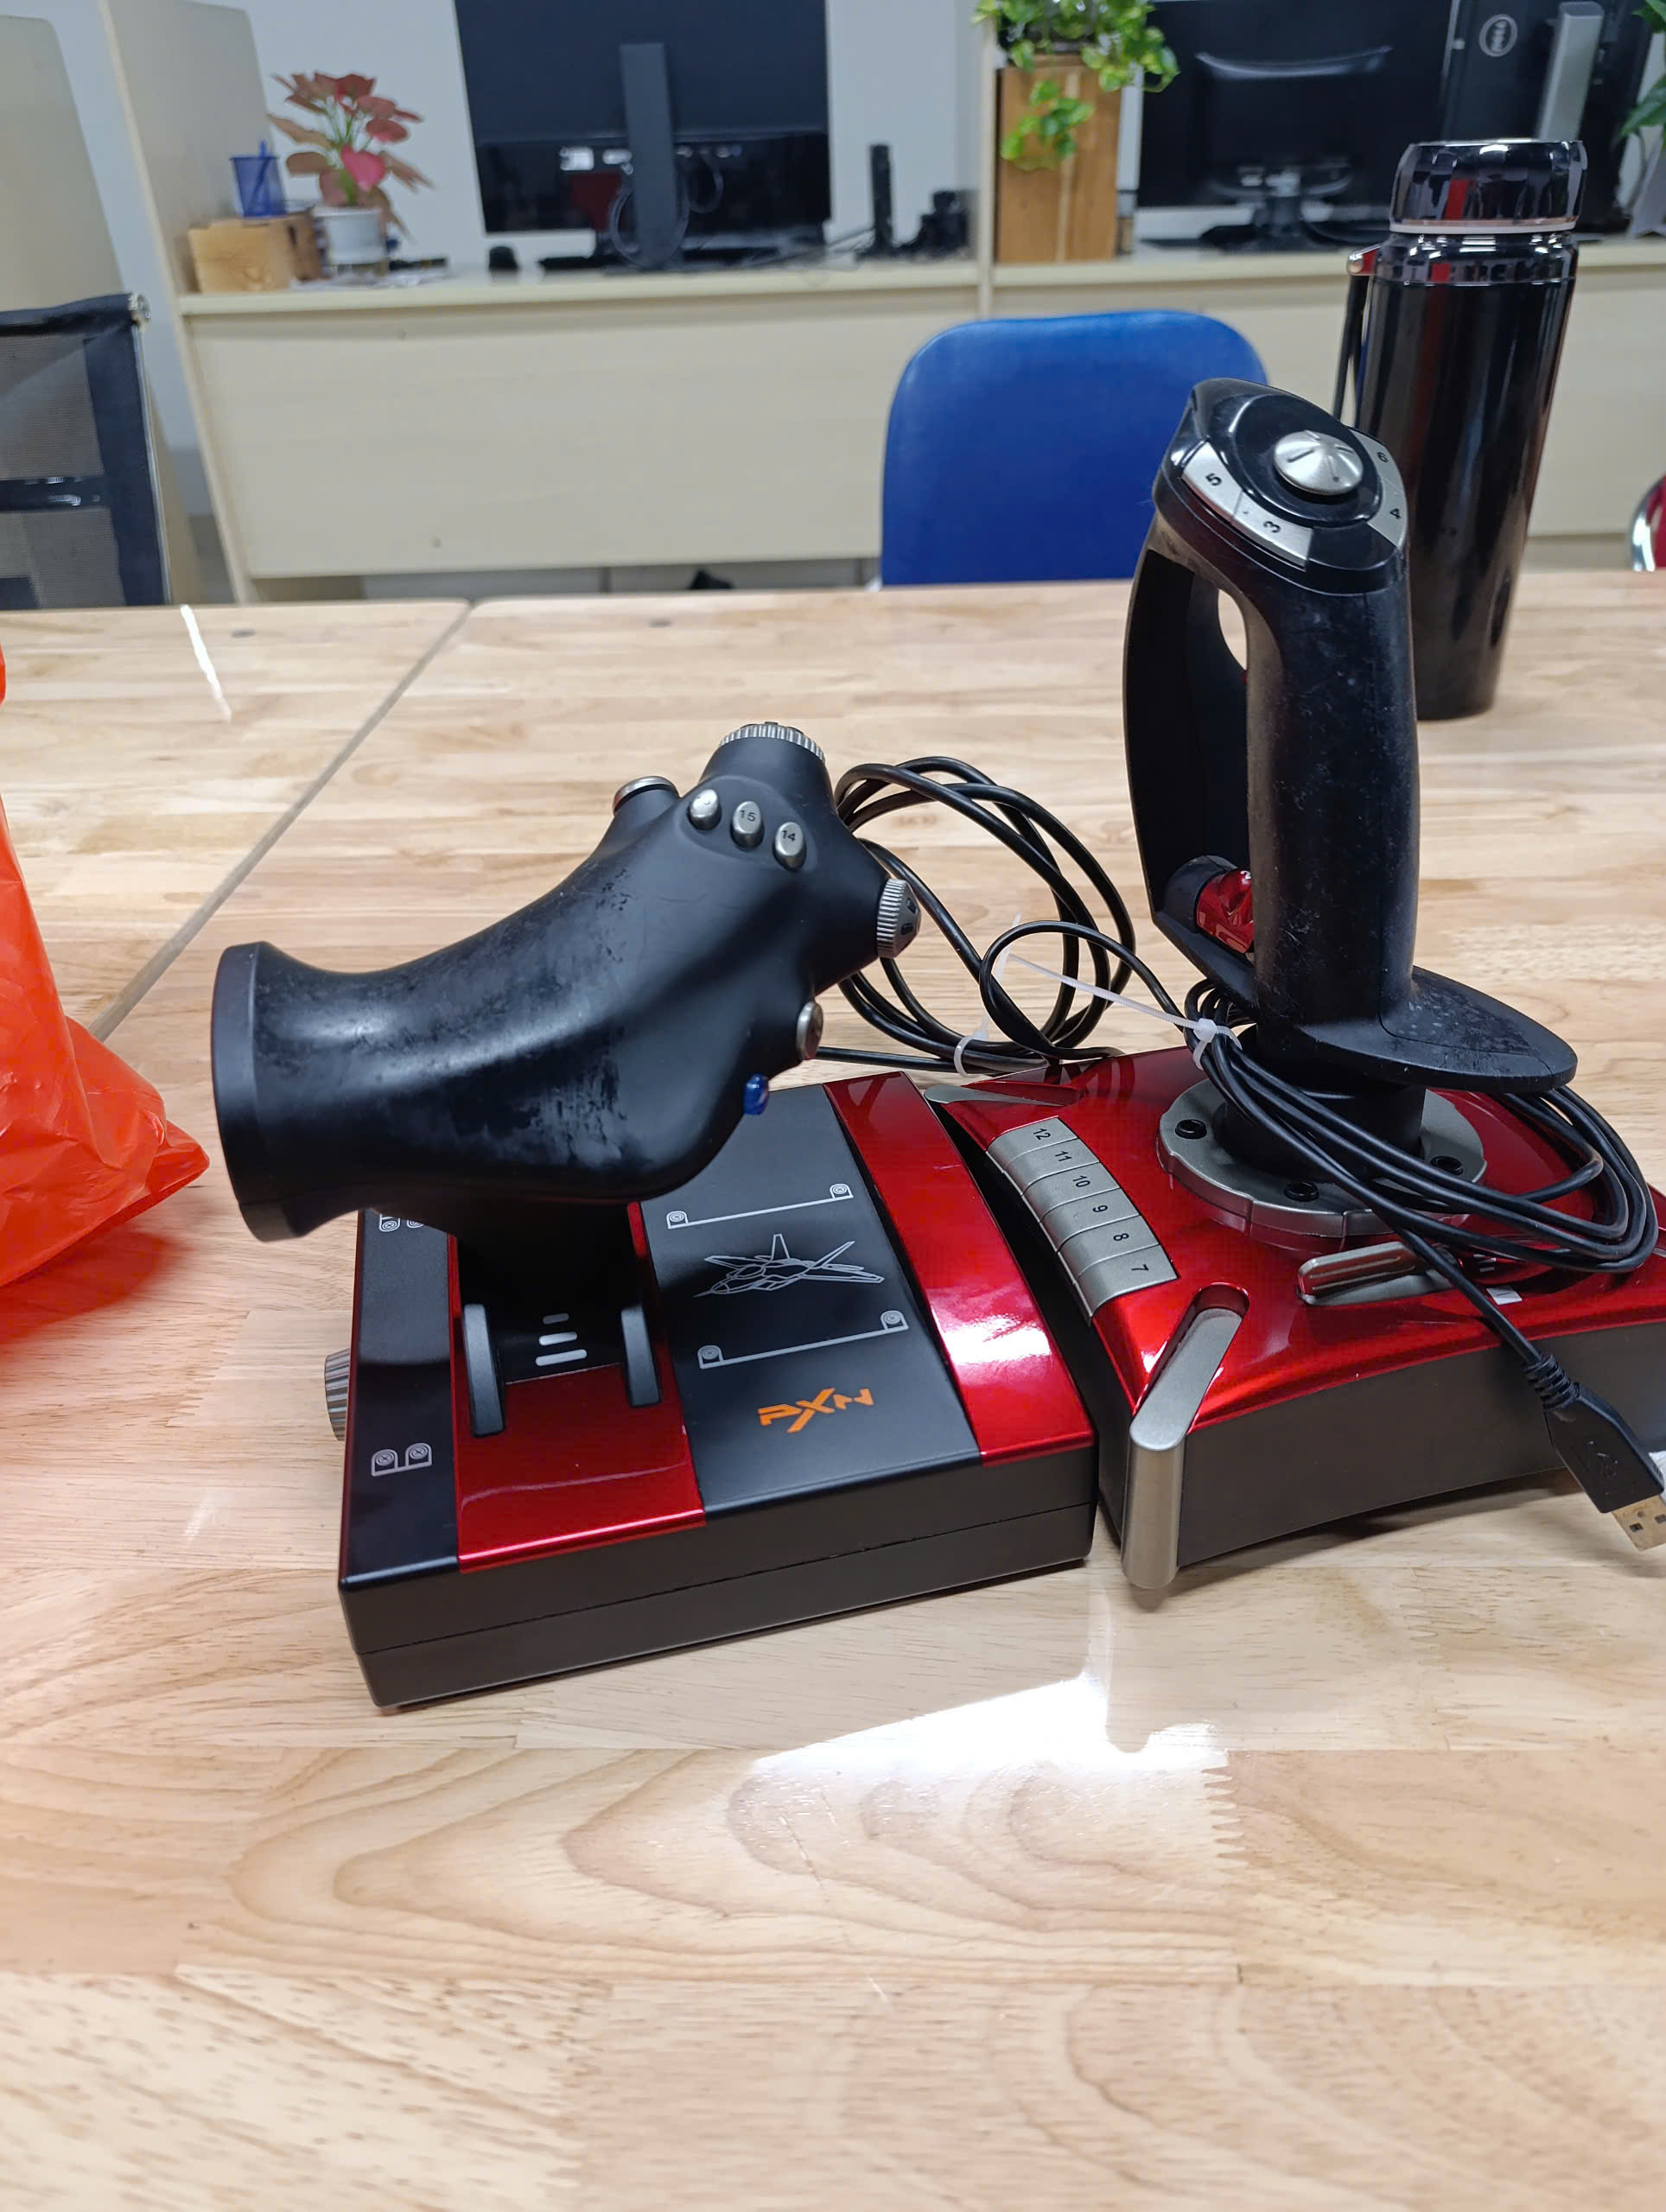
\includegraphics[width=99.91pt,height=99.91pt]{joystick.jpg}};
	%Image [id:dp8812698464016249] 
	\draw (521,112.74) node  {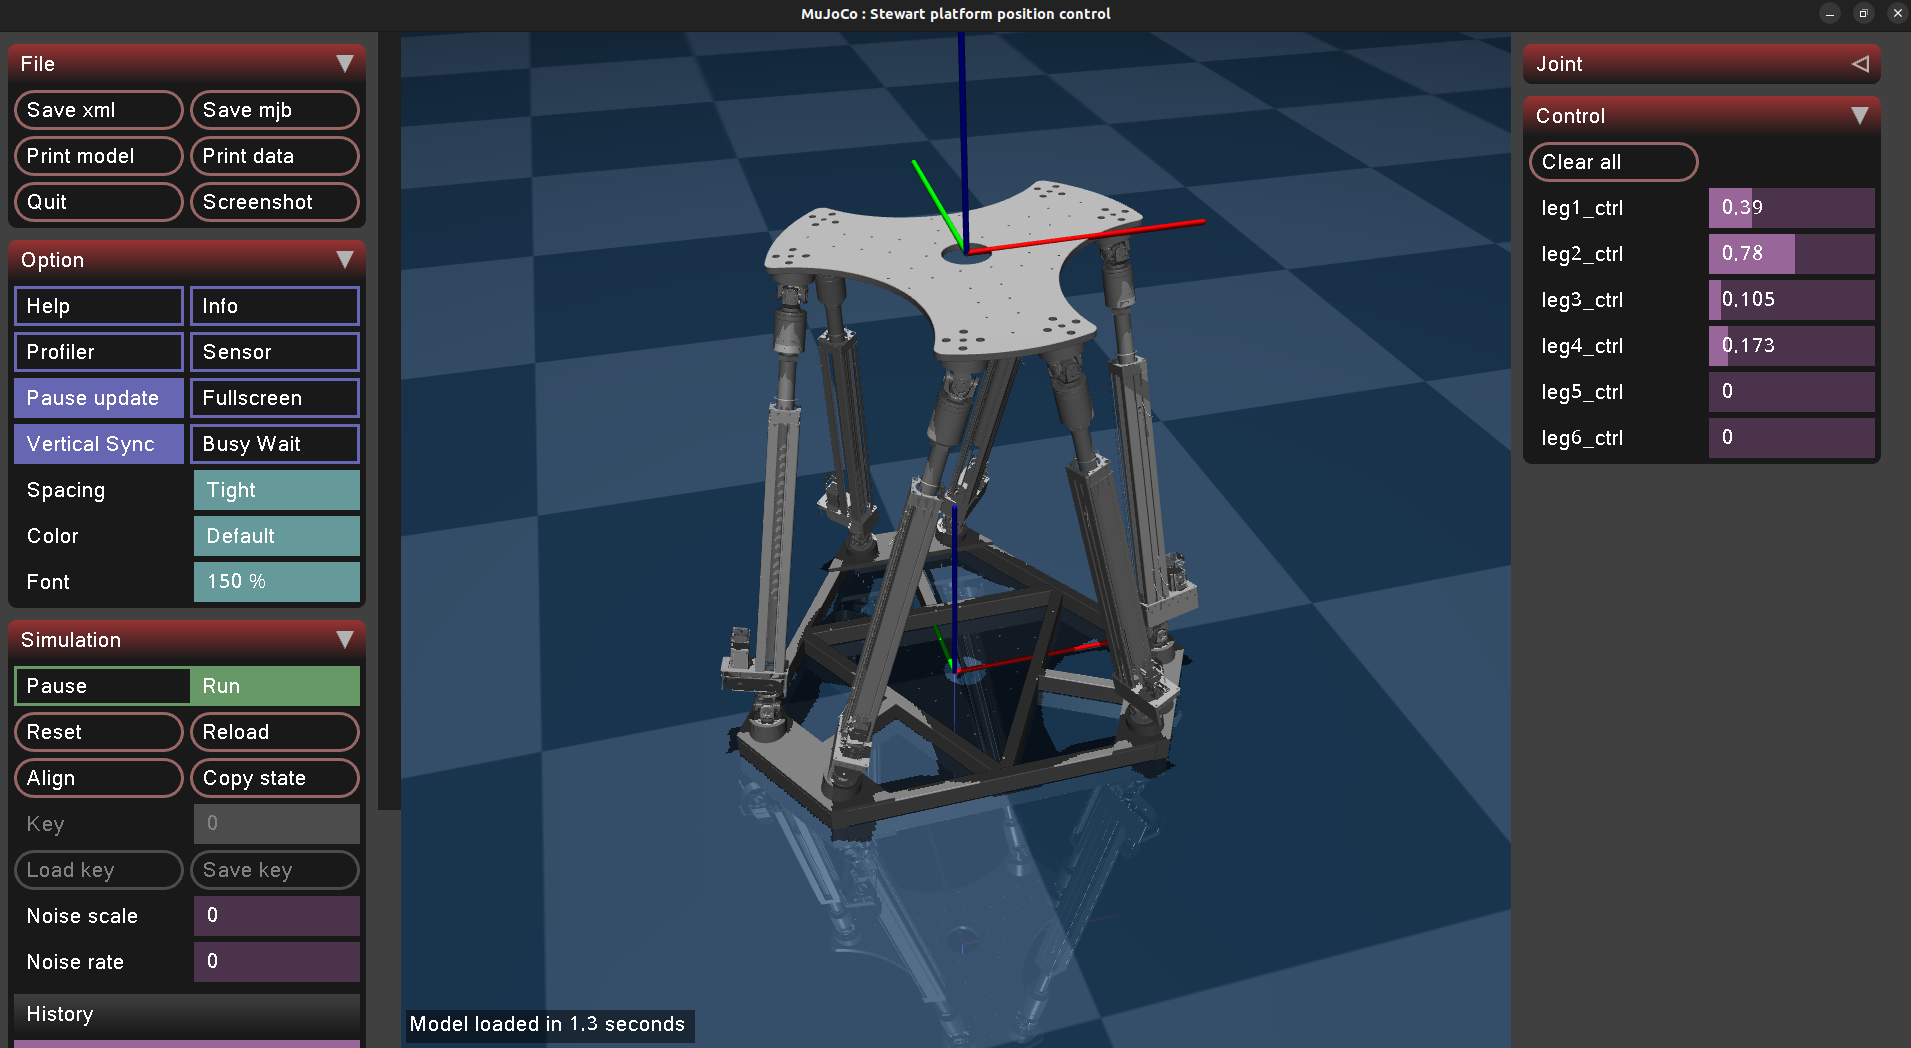
\includegraphics[width=193.5pt,height=106.12pt]{mujoco-stewart.png}};
	%Shape: Rectangle [id:dp8198074648376453] 
	\draw   (392,42) -- (650,42) -- (650,183.49) -- (392,183.49) -- cycle ;
	
	%Right Arrow [id:dp25296009649592344] 
	\draw   (234,146.55) -- (303,146.55) -- (303,140) -- (330,153.1) -- (303,166.21) -- (303,159.66) -- (234,159.66) -- cycle ;
	
	% Text Node
	\draw (180,52) node [anchor=north west][inner sep=0.75pt]   [align=left] {read data from flight joystick};
	% Text Node
	\draw (182,78) node [anchor=north west][inner sep=0.75pt]   [align=left] {evdev};
	% Text Node
	\draw (182,100) node [anchor=north west][inner sep=0.75pt]   [align=left] {pygame};
	
	
\end{tikzpicture}}
			\end{frame}
		
					\begin{frame}[fragile]
			\frametitle{Peripherals connection}
			The source code for this project is not publicly available.
			
			For access or further information, please contact Viet Khanh Nguyen or Duc Cuong Vu.
				\begin{center}
					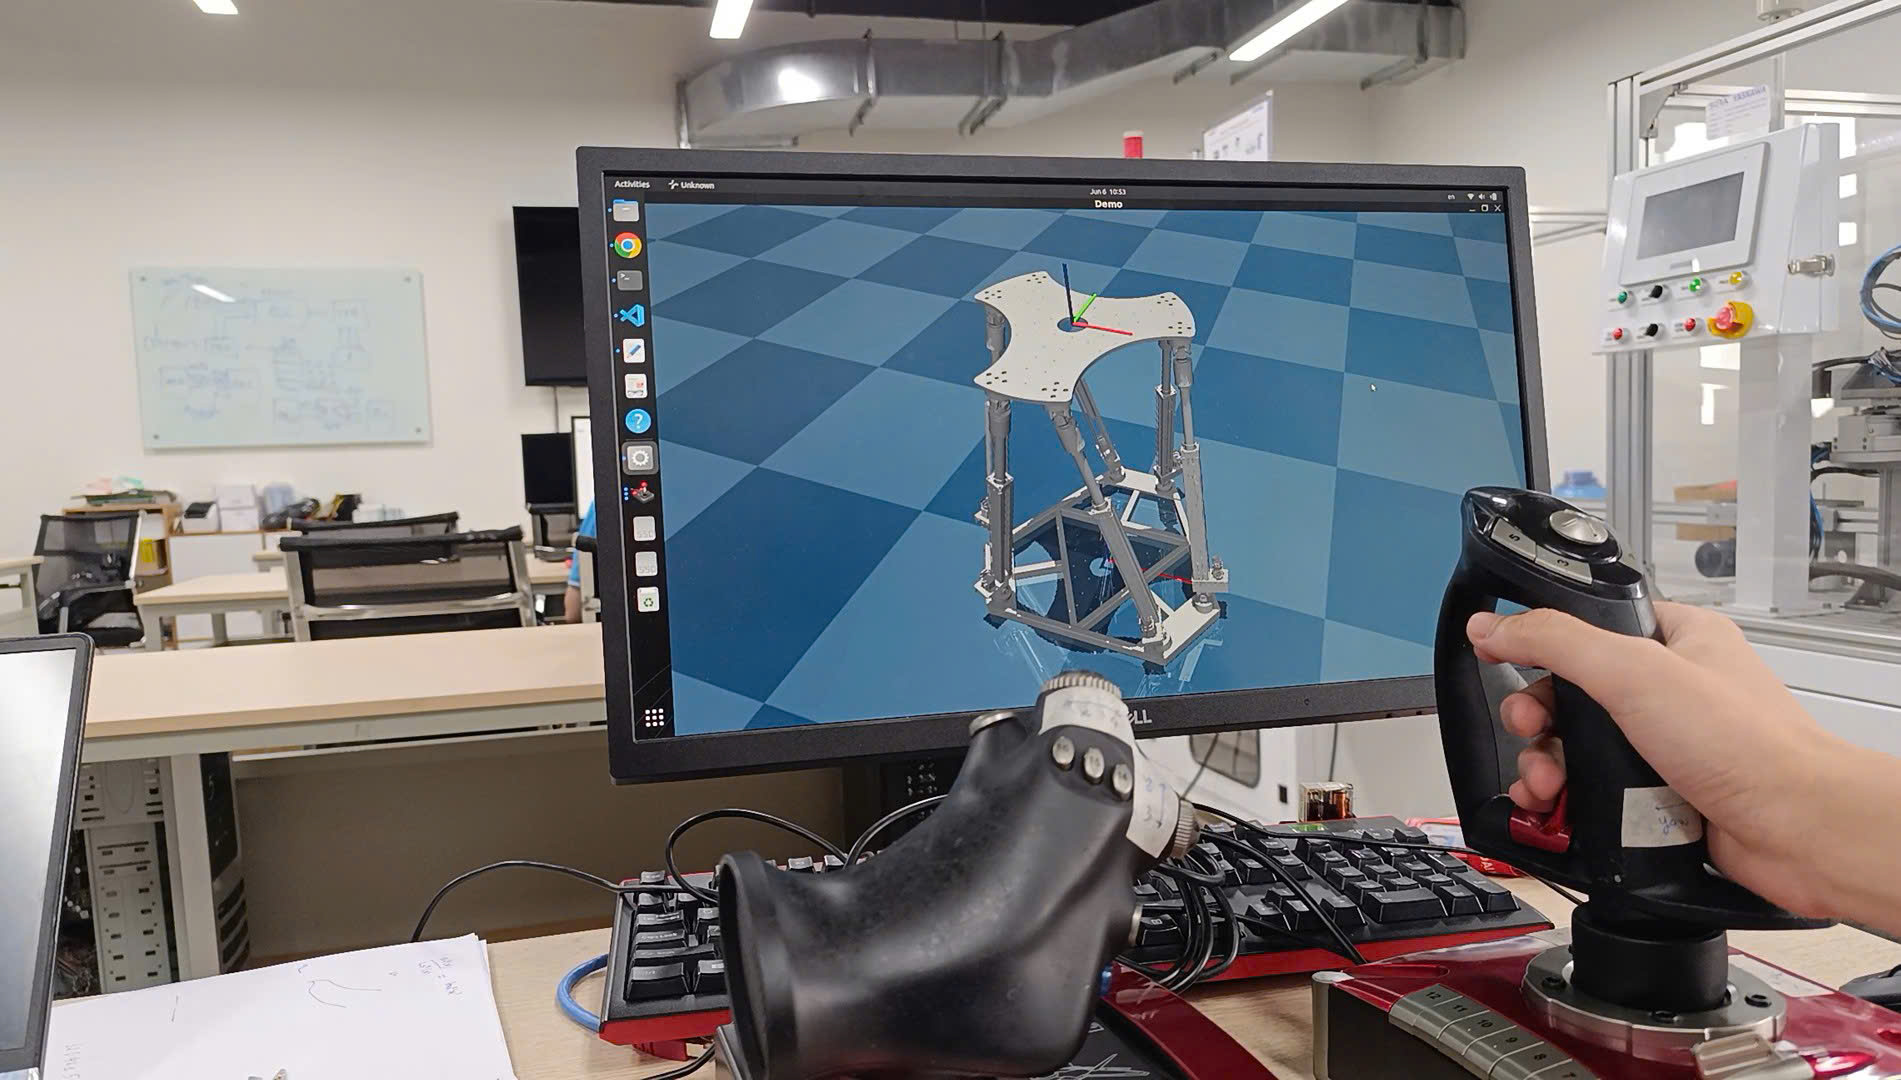
\includegraphics[width=1\linewidth]{images/real-joystick-ctrl}
				\end{center}
				
			\end{frame}
		
		\subsection{Unmanned Aerial Vehicle (UAV)}
			\begin{frame}[fragile]
				\frametitle{Skydio X2 model}
				The model is available at \footnote{text\href{https://github.com/google-deepmind/mujoco_menagerie/blob/main/skydio_x2/x2.xml}{https://github.com/google-deepmind/mujoco\_menagerie/blob/main/skydio\_x2/x2.xml}}
				\begin{center}
					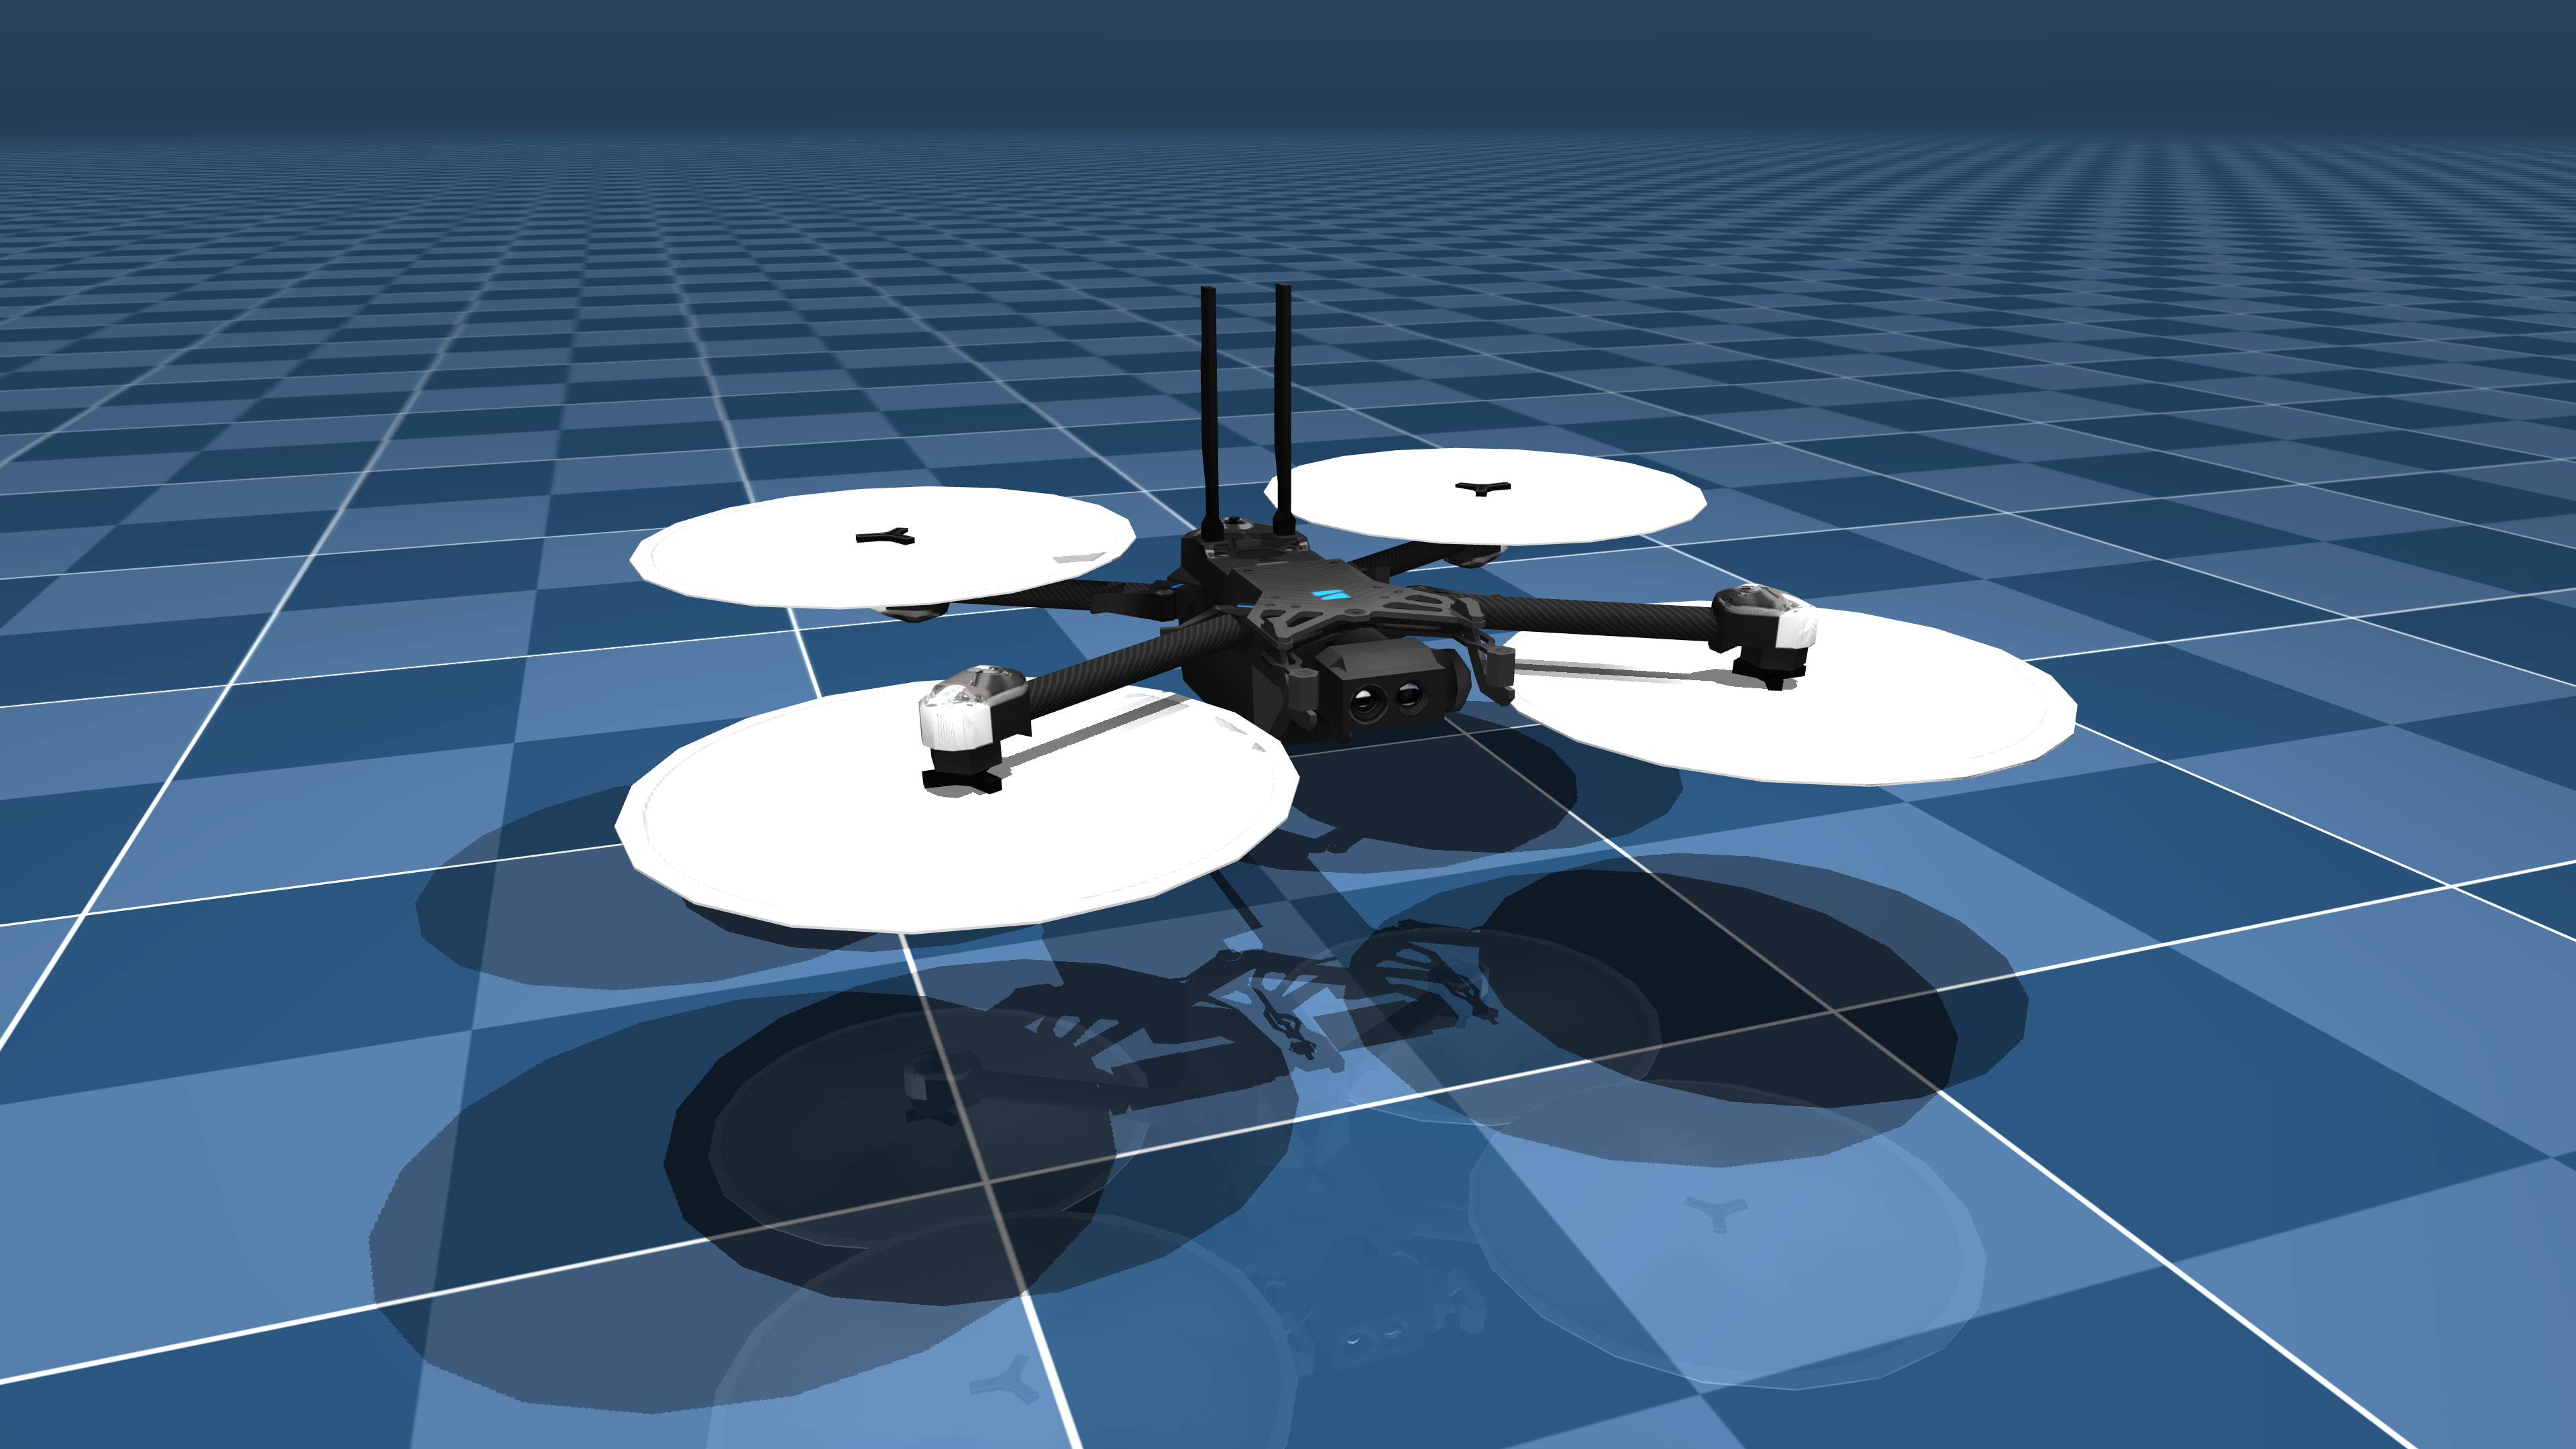
\includegraphics[width=1\linewidth]{images/mjc-x2}
				\end{center}
				
			\end{frame}
		
			\begin{frame}[fragile]
				\frametitle{Skydio X2 model}
				The AUV is a standard model. Actuator allocation can be found in the \texttt{<actuator>} tag below.
				
				In addition, an IMU sensor is used in this model.
					\begin{minted}[fontsize=\footnotesize, linenos, bgcolor=gray!10]{python}
<actuator>
  <motor class="x2" name="thrust1" site="thrust1" gear="0 0 1 0 0 -.0201"/>
  <motor class="x2" name="thrust2" site="thrust2" gear="0 0 1 0 0  .0201"/>
  <motor class="x2" name="thrust3" site="thrust3" gear="0 0 1 0 0  .0201"/>
  <motor class="x2" name="thrust4" site="thrust4" gear="0 0 1 0 0 -.0201"/>
</actuator>

<sensor>
  <gyro name="body_gyro" site="imu"/>
  <accelerometer name="body_linacc" site="imu"/>
  <framequat name="body_quat" objtype="site" objname="imu"/>
</sensor>
				\end{minted}
			\end{frame}
		
			\begin{frame}[fragile]
				\frametitle{Peripherals connection for UAV control}
				The source code for this project is not publicly available.
				
				For access or further information, please contact Viet Khanh Nguyen.
				\begin{center}
					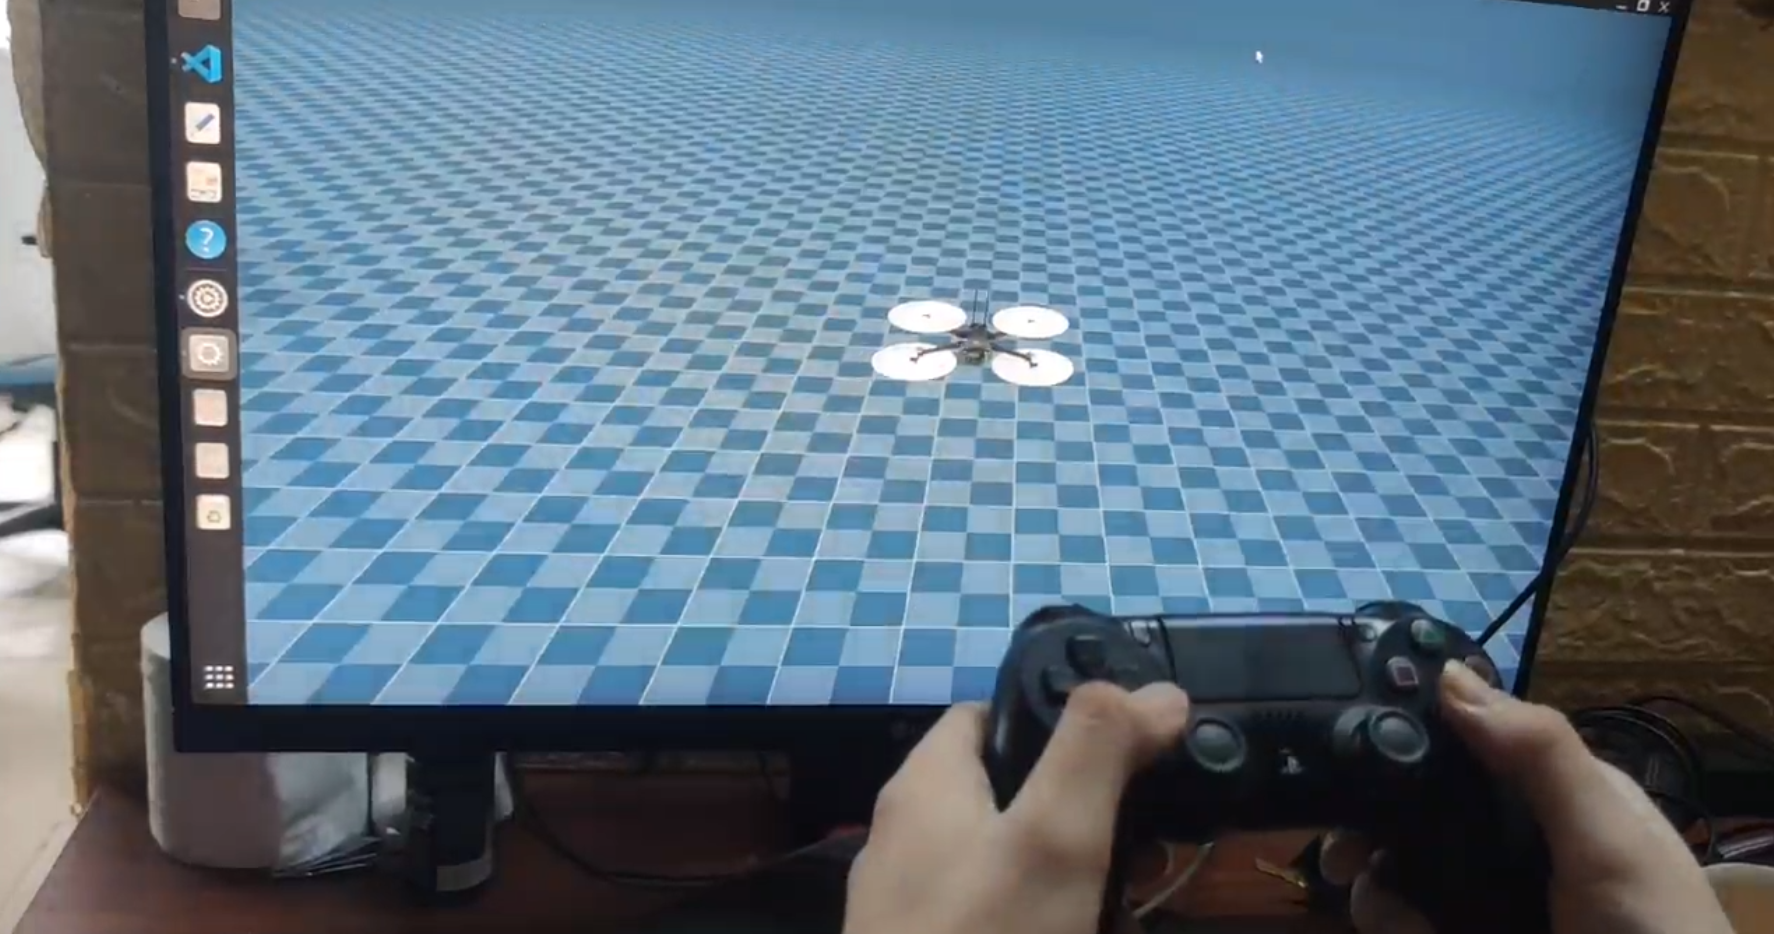
\includegraphics[width=1\linewidth]{images/mjc-uav}
				\end{center}
			\end{frame}
		
		
		
		
		
		\subsection{Autonomous Underwater Vehicle (AUV)}
		
			\begin{frame}[fragile]
				\frametitle{Omni-directional Intelligent Navigation model}
				This repository presents a simulation framework for an Autonomous Underwater Vehicle (AUV) that combines Model Predictive Control (MPC), Control Barrier Functions (CBF) for robust path tracking and obstacle avoidance in dynamic underwater environments. The theories are shown in the publication \footnote{Pham, M. D., Vu, D. C., Nguyen, T. T. H., Nguyen, T. V. A., Vu, M. N., \& Nguyen, T. L. (2025). CBFs-based Model Predictive Control for Obstacle Avoidance with Tilt Angle Limitation for Ball-Balancing Robots. IEEE Access.}
				
				\begin{center}
					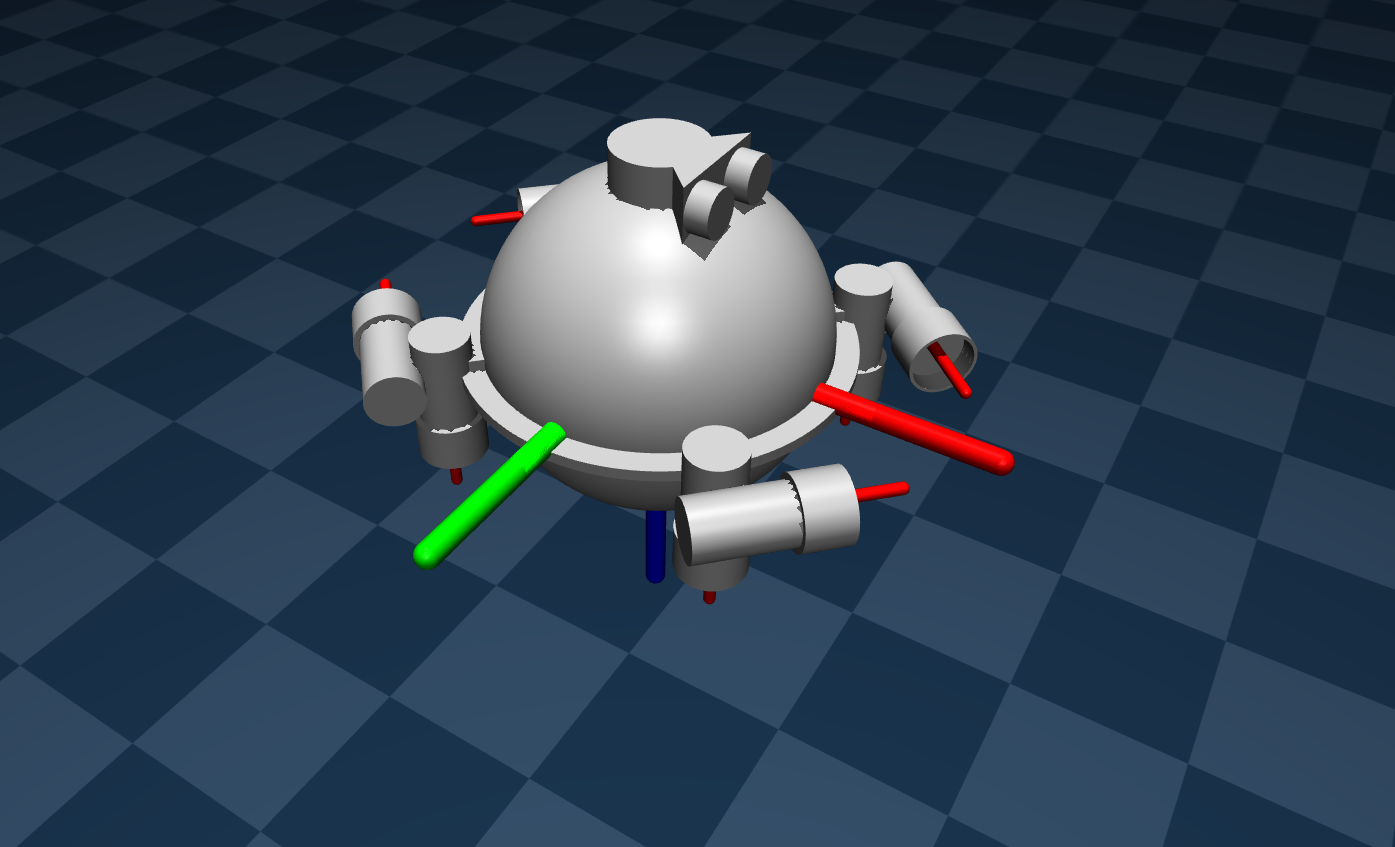
\includegraphics[width=0.5\linewidth]{images/mjc-odin}
				\end{center}
				The source code for this project is not publicly available.
				
				For access or further information, please contact Duc Cuong Vu.
			\end{frame}
		
		
		\begin{frame}[fragile]
			\frametitle{ODIN actuators}
			The ODIN is driven by 8 thruster, it could be defined as follows
				\begin{minted}[fontsize=\footnotesize, linenos, bgcolor=gray!10]{xml}
<actuator>
  <general name = "thruster1" site="thruster1_site" gear="0 0 1 0 0 0"/>
  <general name = "thruster2" site="thruster2_site" gear="0 0 1 0 0 0" />
  <general name = "thruster3" site="thruster3_site" gear="0 0 1 0 0 0" />
  <general name = "thruster4" site="thruster4_site" gear="0 0 1 0 0 0" />
  <general name = "thruster5" site="thruster5_site" gear="0 0 1 0 0 0" />
  <general name = "thruster6" site="thruster6_site" gear="0 0 1 0 0 0" />
  <general name = "thruster7" site="thruster7_site" gear="0 0 1 0 0 0" />
  <general name = "thruster8" site="thruster8_site" gear="0 0 1 0 0 0" />
</actuator>	
			\end{minted}
		and the general force and moment of underwater environment
			\begin{minted}[fontsize=\footnotesize, linenos, bgcolor=gray!10]{xml}
<actuator>
  <general name="Force_X" site="odin_site" gear="1 0 0 0 0 0"/>
  <general name="Force_Y" site="odin_site" gear="0 1 0 0 0 0"/>
  <general name="Force_Z" site="odin_site" gear="0 0 1 0 0 0"/>
  <general name="Moment_K" site="odin_site" gear="0 0 0 1 0 0"/>
  <general name="Moment_M" site="odin_site" gear="0 0 0 0 1 0"/>
  <general name="Moment_N" site="odin_site" gear="0 0 0 0 0 1"/>
</actuator>
		\end{minted}

			
		\end{frame}
			
			
			
			    
			
			\begin{frame}[fragile]
				\frametitle{Optimization-based decision-making}
				Following the SNAME(1950) notation, a general underwater vehicle could be controlled by consider the control input as the forces and moments at the origin. Thus, the force allocation for thruster could be achieved by an energy-optimization decision.
				\begin{minted}[fontsize=\footnotesize, linenos, bgcolor=gray!10]{python}
from scipy.optimize import minimize, Bounds
					
def objective(x):  # Objective: minimize x^T x
	return np.dot(x, x)		
	
def eq_constraint(x):  # Equality constraint: E x = A
	return force_allocation(x) - FandM 		

bounds = Bounds([0, 0, 0, 0, -np.inf, -np.inf, -np.inf, -np.inf], [np.inf]*8)
linear_constraint = {'type': 'eq', 'fun': eq_constraint}

x0 = thurster_prev   # Initial guess

result = minimize(objective, x0, method='SLSQP',
  constraints=[linear_constraint],
  bounds=bounds)
				\end{minted}
			\end{frame}
		
		\begin{frame}[fragile]
			\frametitle{Model Predictive Control with CasADi}
			\begin{minted}[fontsize=\footnotesize, linenos, bgcolor=gray!10]{python}
import casadi as ca
for j in range(N):
  # Apply dynamics to get next state
  x_next = rk4_step(x[:, j], u[:, j], dtc)
  opti.subject_to(x[:, j+1] == x_next)  # Dynamics constraint

  # Tracking error: difference between current position and reference
  e = x[0:3, j] - QR[:, j]
  # Add to cost (only position error considered)
  cost += ca.mtimes([e.T, Q, e])
  # Note: control effort term (u.T * R * u) can be added here

  dist = obs_detected * ((x_next[0] - x_obs)**2 + 
    (x_next[1] - y_obs)**2 + (x_next[2] - z_obs)**2 - r_obs**2)

  # Update obstacle position based on velocity
  x_obs += current_vel[0]*dtc
  y_obs += current_vel[1]*dtc
  z_obs += current_vel[2]*dtc

  # Change in distance between time steps
  diff_dist = dist - dist_before
  dist_before = dist  # Update for next step

  # CBF constraint to ensure distance grows fast enough
  opti.subject_to(diff_dist >= -gamma*dist)
			\end{minted}
		\end{frame}
	
		\begin{frame}
			\frametitle{Model Predictive Control with CasADi}
			\begin{center}
				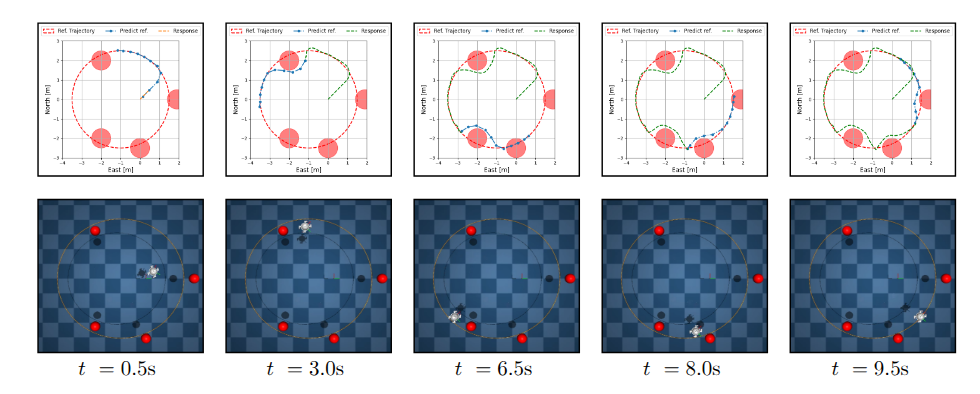
\includegraphics[width=0.9\linewidth, fbox]{images/mjc-odin1m.png}
				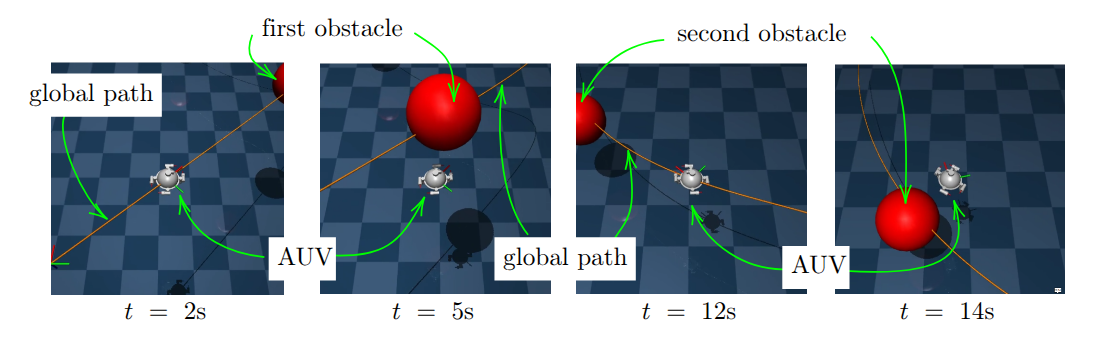
\includegraphics[width=0.9\linewidth, fbox]{images/mjc-odin3.png}
			\end{center}
		\end{frame}
	
		\begin{frame}
			\frametitle{Model Predictive Control with CasADi}
			\begin{center}
				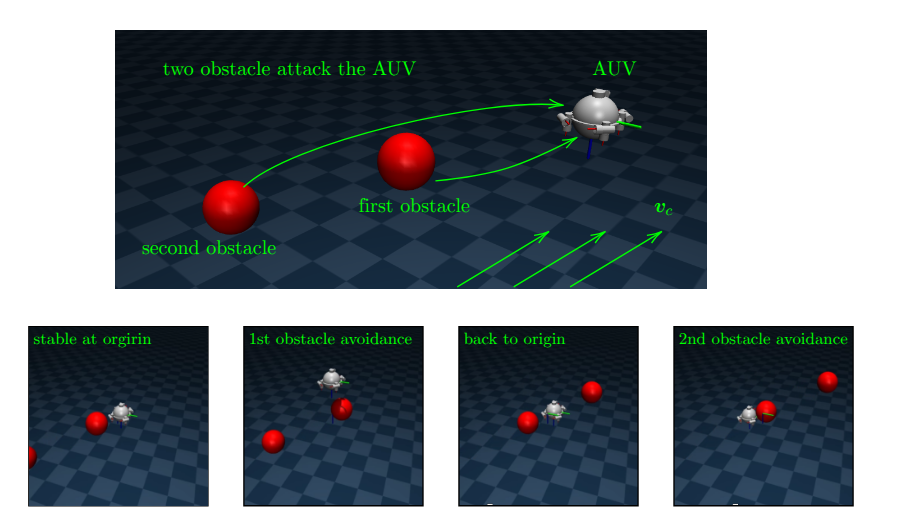
\includegraphics[width=0.9\linewidth, fbox]{images/mjc-odin2.png}
			\end{center}
		\end{frame}
	
		\begin{frame}
			\frametitle{Model Predictive Control with CasADi}
			\begin{center}
				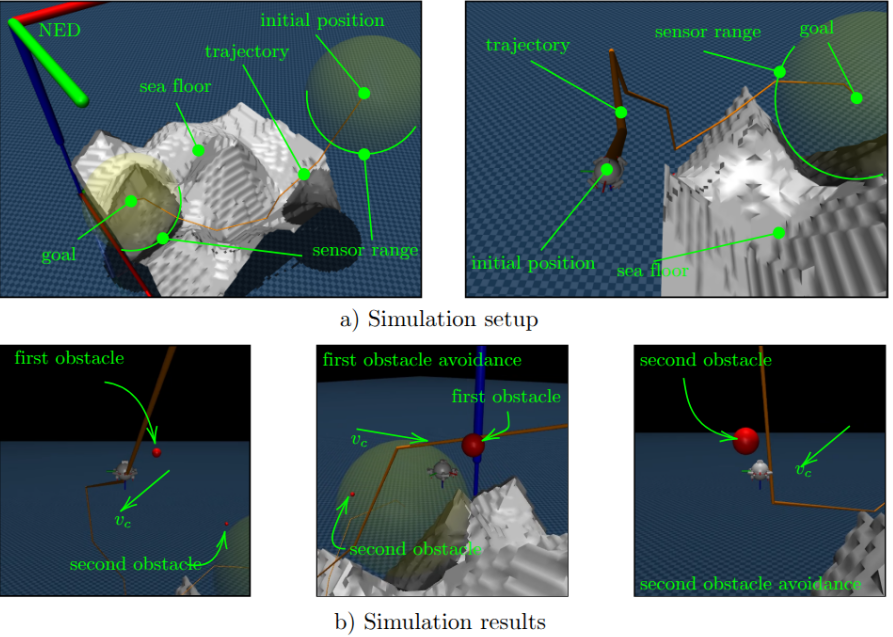
\includegraphics[width=0.9\linewidth, fbox]{images/mjc-odin4.png}
			\end{center}
		\end{frame}
	
	
	% =========================================
	% =========================================
	\section{Q\&A}
	% =========================================
	% =========================================


	
	% =========================================
	% =========================================

	

	
	\begin{frame}{Thanks for your attention! Any questions?}%% 1
		\begin{center}
			\Huge Hope you slept comfortably!
		\end{center}
	\end{frame}
	
\end{document}
